\documentclass{article}
\usepackage[utf8]{inputenc}
\usepackage{graphicx}
\usepackage{amssymb}
\usepackage{tikz}
\usepackage{multicol}
\usepackage{tcolorbox}
\usepackage{multicol}
\usepackage{xcolor}
\usepackage{soul}
\usepackage{amsmath}
\usepackage{pgfplots}
\usepackage{caption}


\usepackage{titlesec}

% Define a new command for subsubsubsection
\titleclass{\subsubsubsection}{straight}[\subsubsection]
\newcounter{subsubsubsection}[subsubsection]
\renewcommand\thesubsubsubsection{\thesubsubsection.\arabic{subsubsubsection}}
\titleformat{\subsubsubsection}[runin]
  {\normalfont\normalsize\bfseries}{\thesubsubsubsection}{1em}{}
\titlespacing*{\subsubsubsection}{0pt}{1ex}{1ex}


\usepackage[linesnumbered, ruled, vlined]{algorithm2e}
\usepackage{inconsolata} % Usa il font Inconsolata per il monospace
\SetAlFnt{\ttfamily} % Imposta il font monospace per l'algoritmo


\graphicspath{ {./paginette/img} }
\tcbuselibrary{breakable}


% color

\definecolor{verdeoscuro}{rgb}{0.0, 0.1, 0.0}
\newcommand{\red}[1]{
    \textcolor{red}{#1}
}

\newcommand{\fab}{
    f : \in [a, b] \rightarrow \mathbb{R}
}
\newcommand{\mathcenter}[1]{
    \begin{center}
        \begin{math}
            #1
        \end{math}
    \end{center}
}
\newcommand{\real}{
\mathbb{R}
}
\newcommand{\reali}{
    $\mathbb{R}$
}

\newcommand{\razionali}{
    $\mathbb{Q}$
}

\newcommand{\definizione}[1]{
    \begin{tcolorbox}[colback=orange!10!white,  colframe=orange!50!black, colframe=white, sharp corners, title=Definizione]
        #1
    \end{tcolorbox}
}

\newcommand{\esempio}[1]{
    \begin{tcolorbox}[colback=green!10!white, colframe=white, sharp corners, breakable]
        #1
    \end{tcolorbox}
}

\newcommand{\dimostrazione}[1]{
    \begin{tcolorbox}[colback=blue!10!white, colframe=blue!50!black, title= dimostrazione, breakable]
    
    #1
    \end{tcolorbox}
}

\newcommand{\teorema}[1]{
\begin{tcolorbox}[colback=violet!10!white, colframe=violet!50!black, title= teorema, breakable]
#1
\end{tcolorbox}
}

\newcommand{\lemma}[1]{
\begin{tcolorbox}[colback=yellow!10!white, colframe=yellow!50!black, title= lemma, breakable]
#1
\end{tcolorbox}
}

%title





\begin{document}
\tableofcontents


\chapter{I numeri finiti}
\section{Base-N and Binary}

I numeri hanno diversi modi per essere rappresentati, tra cui quello più comune che è la \textbf{rappresentazione decimale}, dove ogni numero è formato da una lista di caratteri compresi tra $[0,9]$ dove ad ogni cifra è associata una potenza del 10
\\
\esempio{
    \textbf{Esempio}: $147.3 = 1 \cdot 10^2 + 4 \cdot 10^1 + 7 \cdot 10 ^0 + 3 \cdot 10^{-1}$ 
}

In generale, comunque, per convertire un numero da una base \textit{n} a base 10:
\teorema{
    Dato un numero in base \(n\) \( (a_k a_{k-1} \dots a_1 a_0)_n \), la sua conversione in base 10 è data dalla formula:

    \[
    \sum_{i=0}^{k} a_i \cdot n^i
    \]

    dove \(a_i\) sono le cifre in base \(n\) e \(n\) è la base.

}

Per forza di cose i calcolatori operano con i numeri \textit{in base 2}, le cui cifre vengono chiamate\textbf{bit}, esempio $101101$ (base 2).
Per convertire un numero dalla base 10 alle base bisogna dividerlo in potenze di due 
\esempio{
    \[
        37 \, (\text{base } 10) = 32 + 4 + 1 = 1 \cdot 2^5 + 0 \cdot 2^4 + 0 \cdot 2^3 + 1 \cdot 2^2 + 0 \cdot 2^1 + 1 \cdot 2^0 = 100101 \, (\text{base } 2)
    \]
}

In generale occorre dividerlo per due finchè non si riduce ad uno ad esempio: 
\[
(35)_{10} = (100011)_2
\]

\begin{align*}
    35 : 2 &= 17 \quad \text{resto } 1 \\
    17 : 2 &= 8  \quad \text{resto } 1 \\
    8 : 2  &= 4  \quad \text{resto } 0 \\
    4 : 2  &= 2  \quad \text{resto } 0 \\
    2 : 2  &= 1  \quad \text{resto } 0 \\
    1 : 2  &= 0  \quad \text{resto } 1
    \end{align*}
    
    % Creiamo la freccia accanto a tutto l'insieme di divisioni
    \begin{tikzpicture}[overlay, remember picture]
        \draw[->, red, thick] (5.5,1) -- (5.5,-5.5);
    \end{tikzpicture}


\subsection{Addizione e moltiplicazione in binario}
\subsection{Conversione fra basi}
\subsection{Floating point}
Data la finitezza della memoria di un calcolatore, e' impossibile rappresentare esattamente un numero che ha precisione infinita. Per riuscire a rappresentare in modo piu' efficente possibile si usano i \textbf{floating point} numbers:
\dfn{Floating Point}{
  Alloca:
  \begin{itemize}
    \item Un indicatore per il segno ($ s $)
  \item L'esponente ($ e $)
  \item La mantissa ($ f $)
  \end{itemize}
}

Nello standard \textbf{IEEE754} double precision, che occupa 64 bit, un numero e' rappresentato nel seguente modo:
\begin{center}
    no puede soportar este sufrimento
  %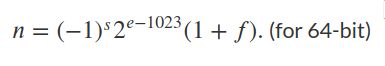
\includegraphics[width=0.5\textwidth]{img/2024-09-16-14-02-10.png}

\end{center}

In generale, ogni numero reale $ n \in \mathbb{R} $ e' definito da:
\begin{center}
    no puede soportar este sufrimento
  %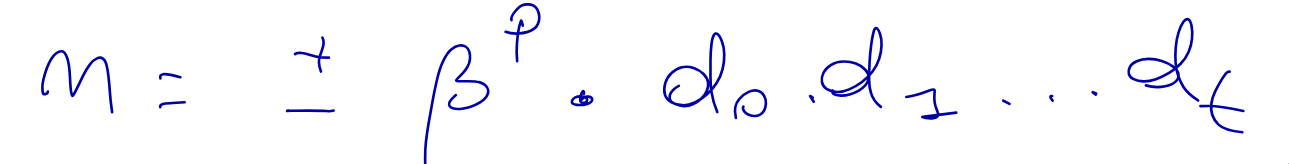
\includegraphics[width=0.5\textwidth]{img/2024-09-16-14-03-42.png}
\end{center}

Quindi l'insieme dei numeri floating point caratterizzati dai valori $ \beta, t, +L, U $ sono:
\begin{center}
    no puede soportar este sufrimento
  %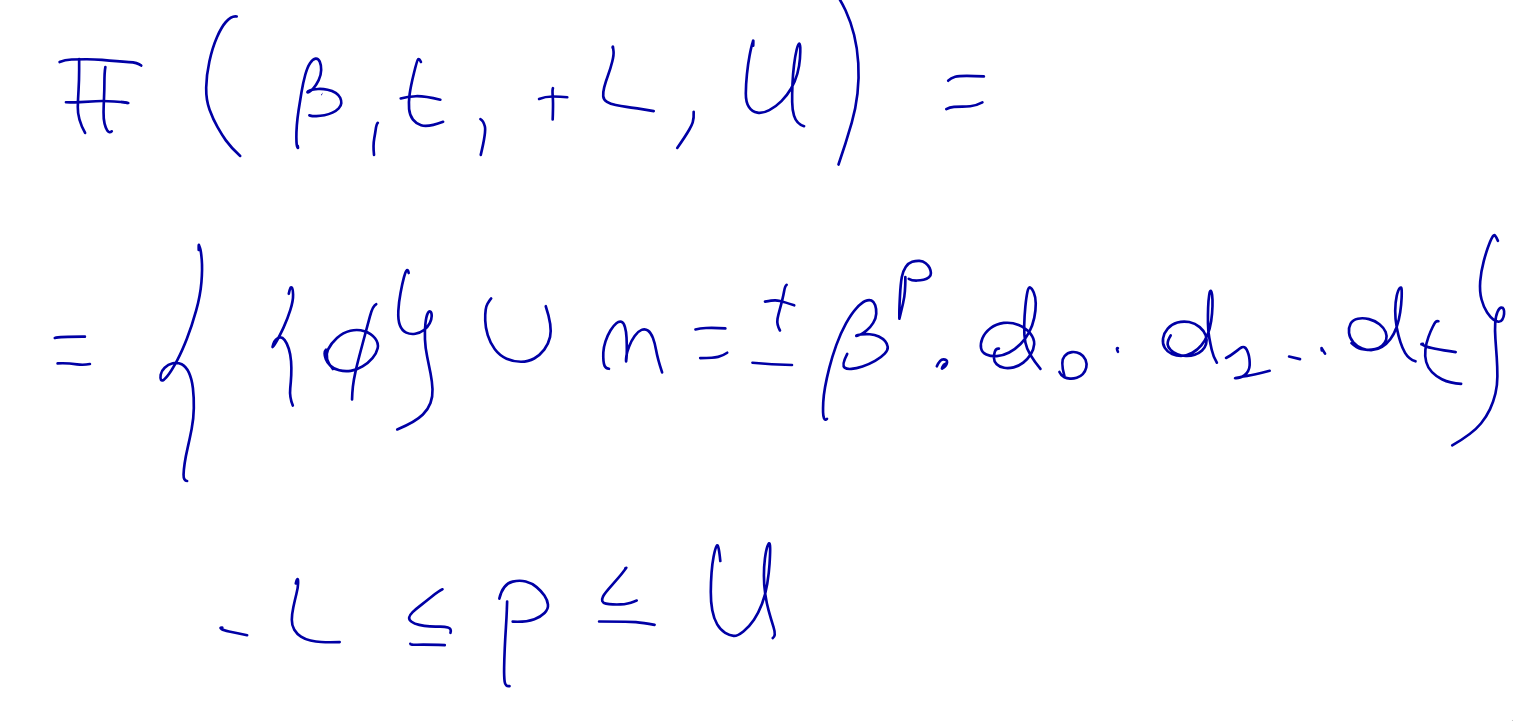
\includegraphics[width=0.5\textwidth]{img/2024-09-16-14-09-02.png}

\end{center}

Se un numero $ x \in \mathbb{R} $ ha un numero di cifre decimali maggiore di $ t $, allora $ x \not\in \mathcal{F} $ e deve essere approssimato (solitamente col troncamento).

\section{Errori di rappresentazione}
Dato che stiamo usando lo stesso numero di bit, il numero di valori rappresentabili rimane uguale, ma la codifica \textit{floating point} fa in modo che il \textbf{gap}, ovvero la differenza, fra due numeri successivi (che esistono sempre dato che lavoriamo con valori discreti) sia relativo al valore assoluto dei numeri rappresentati. Questo e' utile dato che riusciamo ad essere molto precisi con numeri piccoli, riuscendo comunque a rappresentare valori enormi con un errore che in confronto rimane minuscolo. 
\begin{center}
    no puede soportar este sufrimento
  %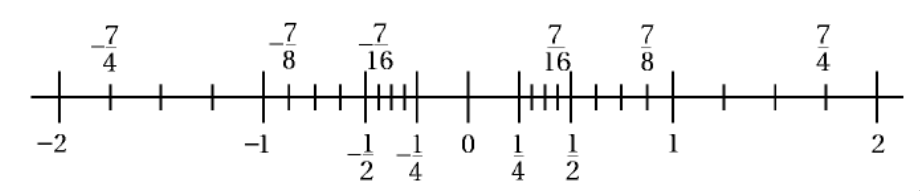
\includegraphics[width=0.5\textwidth]{img/2024-09-22-16-37-40.png}

\end{center}
Abbiamo due modi per indicare l'accuratezza con la quale possiamo rappresentare un valore $ x \in \mathbb{R} $:
\begin{itemize}
\item L'errore \textbf{assoluto}, che e' piu' grande piu' e' grande l'ordine di $ x $
  \[
    |fl(x)-x|<\\beta^{p-t}
  \]
\item E quello \textbf{relativo}, che dipende solo da $ t $
  \[
    \frac{|fl(x)-x|}{|x|} < \frac{1}{2}\beta^{1-t} = \text{\textbf{eps}}
  \]
\end{itemize}
Il valore \textbf{eps} e' detto \textbf{precisione macchina}, ed e' il numero macchina piu' piccolo positivo tale che
\[
  fl(1+\text{eps}) > 1
\]
Quindi, definite due operazioni generiche, una per i reali e l'altra per i floating-point:
\begin{itemize}
\item $ \cdot: \mathbb{R} \times \mathbb{R} \to \mathbb{R} $
\item $ \circ: \mathbb{F} \times \mathbb{F} \to \mathbb{F} $
  \[
    x \circ y = fl(x \cdot y)
  \]
\end{itemize}
Abbiamo che ogni operazione fra floating-point genera un errore (di \textbf{arrotondamento}):
\[
  \left|\frac{(x \circ y) - (x \cdot y)}{x \cdot y}\right| < \text{eps}
\]  
Nel caso di somma di numeri di grandezza molto diversa, le cifre piu' significative del numero piu' piccolo possono essere perse. Per una sola operazione questo non causa un errore troppo grande, ma se l'operazione viene eseguita molte volte l'errore si \textbf{amplifica} e puo' diventare catastrofico.

\section{hklklk}

\subsection{Che cos'è il floating point}
Dato che in informatica non è possibile implementare il concetto di infinito (a differenza della matematica) non si è in grado di rappresentare tutto l'insieme dei reali; pertanto occorre, per forza di cose, approssimarlo. Il metodo che oggi è comune per il calcolo scientifico è noto come sistema \textbf{floating point} che permette una rappresentazione di ampio intervallo della retta reale con una distribuzione uniforme degli errori 


\subsection{Definizione formale}
\definizione{
    Si definisce \textbf{inseime dei numeri numeri macchina}  (floating point) con $t$ cifre significative, con base $\beta$, con $p \in [L,U]$ e con le cifre $d_i$ dove $0 \leq d_i \leq \beta -1$, $i = 1, 2, \dots$ e $d_1 \neq 0$
    \[
        \mathbb{F}(\beta, t, L, U) =  \{ 0 \} \cup \{ x \in \mathbb{R} = \text{sign}(x) \beta^{p} \sum_{i=1}^{t} d_i \beta^{-i} \}
    \]
    Usualmente $U$ è positivo e $L$ negativo
}

Questo insieme è, quindi, un'approssimazione all'intervallo preciso di numeri $[min, max] \subseteq \mathbb{R}$ che dipendono da $U$ e $L$. Se voglio rappresentare un numero maggiore/minore di questo intervallo avrò un errore chiamato \textbf{overflow/underflow}



\subsection{Gap}
con questa notazione non è impossibile scrivere ogni numero presente nella retta dei numeri Reali $\mathbb{R}$, ma tra due numeri vi è sempre una certa distanza quindi è pertanto vero che $\mathbb{F}\subseteq \mathbb{R}$. Questo concetto introduce la definizione di Gap:
\definizione{
    Chiamiamo \textbf{gap} la distanza da un numero al suo sucessivo
}
È, inoltre, vero che il gap rimane costante quando l'esponente non cambia, mentre se nell'insieme $\mathbb{F}$ il sucessivo di un numero ha un espente diverso il suo gap sarà diverso di quello del suo precedente con l'esponente uguale. Facciamo un esempio per rendere il tutto più chiaro:
\esempio{
    Sia $\beta = 2, t = 3, L = -1, U=2$ allora
    \[
        \mathbb{F}(2,3,-1,2) = \{0\}\cup\{0.100\times2^p, 0.101\times2^p, 0.110\times2^p,0.111\times2^p, p = -1, 0,1,2\}
    \]
    Questo insieme rappresenta 33 nuemri compreso lo 0:

    %! RIFARE BENE
    \begin{multicols}{4}
        \[
        \begin{array}{c}
        .100(-1) \\
        \frac{1}{4} \\
        .100(0) \\
        \frac{1}{2} \\
        .100(1) \\
        1 \\
        .100(2) \\
        2
        \end{array}
        \]
        \columnbreak
        \[
        \begin{array}{c}
        .101(-1) \\
        \frac{5}{16} \\
        .101(0) \\
        \frac{5}{8} \\
        .101(1) \\
        \frac{5}{4} \\
        .101(2) \\
        \frac{5}{2}
        \end{array}
        \]
        \columnbreak
        \[
        \begin{array}{c}
        .110(-1) \\
        \frac{6}{16} \\
        .110(0) \\
        \frac{6}{8} \\
        .110(1) \\
        \frac{6}{4} \\
        .110(2) \\
        \frac{6}{2}
        \end{array}
        \]
        \columnbreak
        \[
        \begin{array}{c}
        .111(-1) \\
        \frac{7}{16} \\
        .111(0) \\
        \frac{7}{8} \\
        .111(1) \\
        \frac{7}{4} \\
        .111(2) \\
        \frac{7}{2}
        \end{array}
        \]
    \end{multicols}
    La rappresentazione di $\mathbb{F}$ nella retta dei numeri reali è questa
    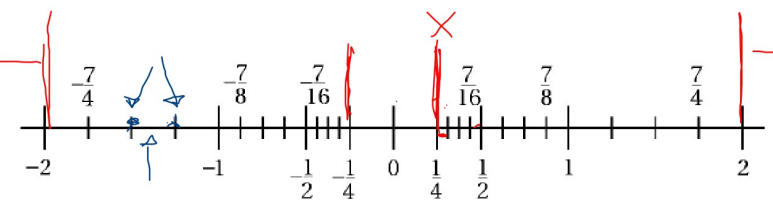
\includegraphics[width=10cm]{retta_reale.png}
}

Risulta quindi evidente l'aumento dell'ampiezza degli intervalli definiti dal valore $p$, in ognuno dai quali vengono localizzati le $t$ cifre della mantissa; ne risulta di conseguenza una diradazione delle suddvisioni verso gli estremi sinistro e destro della retta reale. \\
Il numero $t$, quindi, fissa la precisione di rappresentazione di ogni numero; infatti la retta viene suddivisa in intervalli $[\beta^p,\beta^{p+1}]$  di ampiezza crescente e in questi intervalli viene vengono rappresentati lo stesso numero $(\beta-1)\beta^{t-1}$ di valori, generando ,così, una suddivisione molto densa per valori vincini allo 0 e più rada per valori grandi in valore assoluto. Di conseguenza si ha che \textbf{maggiore è il numero $t$ di cifre della mantissa, minore sarà l'ampiezza dei intervalli e quindi migliore l'approssimazione introdotta}

\subsection{floating point nei calcolatori}
La rappresentazione più comune del sistema nei calcolatori è definita dallo Standand IEEE 745 il cui insieme è $\mathbb{F}(2,52,1023,1024)$ ed è descritta dalla formula
\[
    n = (-1)^s \cdot 2^{e-1023} \cdot (1+f)   
\]

Dove: 
\begin{itemize}
    \item \textbf{s}: è un bit che determina il segno del numero. Se $s=0$ il numero è positivo, se $s=1$ il numero è negativo.
    \item \textbf{e}: è l'esponente del numero due, ed è un intero di 11 bit tale che $e \in [0,2047]$.
    \item \textbf{f}: il valore detto \textbf{mantissa} è una serie di 52 bit che rappresenta la parte frazionaria del numero, nel nostro caso $f \in [0,1]$.
    \item \textbf{1023}: è detto \textbf{bias} ed è usato per codificare esponenti negativi e positivi.
\end{itemize}
In memoria si traduce in un array contentente questi bit:
\begin{center}
    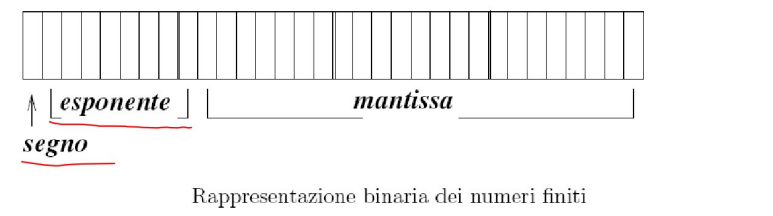
\includegraphics[width=7cm]{floating_point_in_memoria.png}
\end{center}

\esempio{
    Per trovare la codifica del numero in floating point 1 10000000010 1000000000000000000000000000000000000000000000000000 in base 10 occorre:
    \begin{enumerate}
        \item Trovare l'esponente decimale, che è $1 \times 2^{10} + 1 \times 10^1 - 1023 = 3$.
        \item Trovare la parte frazionaria, che è $1 \times \frac{1}{2^1} = 0,5$.
    \end{enumerate}

    Quindi $n = (-1)^1 \times 2^3 \times (1+0,5) = -12,0$.
}

\subsection{troncamento}

Sia l'insieme $\mathbb{F}(\beta, t, L, U) =\{ \{\emptyset\} \cup n = \pm \beta^p \cdot d_0 d_1 \dots d_t  \} $ con $-L \leq p \leq U$ l'insieme dei numeri floating point caratterizzati dai valori $\beta, t, L, U$

Inoltre sia $x \in \mathbb{R}$ dove $x = \pm \beta^p \cdot d_0 d_1 \dots d_t, d_{t+1}, \dots$ con $L\leq p \leq U$, nel caso in cui $x \notin \mathbb{F} $ rappresento $x$ con un elemento di $\mathbb{F} $ che indico con $fl(x) = \pm \beta^p \cdot d_0 d_1 \dots d_t$. Questa operzione si chiama \textbf{troncamento}

\subsection{Errore relativo di arrotondamento}
Il sistema floating point dato che è un'approssimazione è ovvio che la precisione di rappresentazione che offre non è perfetta, in quanto i numeri infiniti (come il $\pi$) vengono delineati con una serie finita di numeri finiti. La differenza tra la sua approssimazione e il suo valore reale è detta \textbf{errore di arrotondamento}  
\subsubsection{definizione}
klkjlkjkljlkj
\definizione{
    Sia $x\in \mathbb{R}$ un numero reale e sia $fl(x)$ (dove $fl()$ è la funzione arrotondamento) il numero $x$ arrotondato, allora l'errore realtivo di arrotondamento è definito dalla seguente formula:
    \[
        \frac{|fl(x)-x|}{|x|} \leq \frac{1}{2}\beta^{1-t}
    \]
}
 La quantità $esp=\frac{1}{2}\beta^{1-t}$ è detta  \textbf{precisione macchina} nel sistema floating point, ed è il più piccolo numero macchina positivo tale che: 
 \[
    fl(1+esp)>1
 \]

\subsection{artimetica floating point}
Il calcolatore esegue operazioni solo con numeri rappresentabili da calcolatore stesso, quindi in questo caso dai numeri scritti in forma floating ponti (per i nuemri reali), il punto è che \red{le usuali operazioni aritmetiche non sono chiuse nell'insieme $\mathbb{F}$}, quindi presi 2 numeri dall'insieme $\mathbb{F}$ e computati tramite operazioni aritmetiche, il risultato di tale computazione potrebbe appartenere nell'insieme $\mathbb{R}$. Pertanto \red{i risultati delle varie computazioni dovranno essere sempre arrotondati ad un numero che stia in $\mathbb{F}$}
\subsubsection{operazione floating point} 
L'operazione floating point (o di macchina) è definita
\definizione{
    \[
        \odot :\mathbb{R}\times\mathbb{R}\rightarrow\mathbb{R}
    \]
}
Ogni operazione provoca un piccolo errore detto \textbf{errore di arrotondamento}:
\[
    |\frac{(x\odot y)-(x\cdot y)}{x\cdot y}|<eps
\]

l'operazione floating point nei calcolatori viene strutturata in due fase:
\begin{enumerate}
    \item \textbf{Eseguo l'operazione esatta}: (es. $z=x+y$) dove viene fatta utilizzando più bit utilizzati di quelli utilizzati per memorizzare il risultato, non è accessibile all'utente ma viene memorizzato in un registro interno alla cpu
    \item \textbf{Trocamento del risultato}: (es. $x\oplus y = fl(z)$), dove una volta che il calcolo è stato fatto in precisione estesa il risultato viene arrotondato alla precisione del risultato
\end{enumerate}
\esempio{
    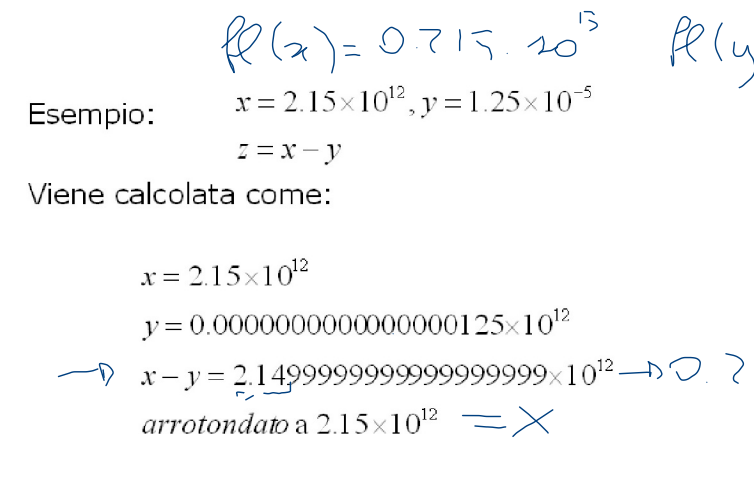
\includegraphics[width=10cm]{arrotondamento_esempio.png}
}

\chapter{Sistemi lineari}

\section{Algoritmi per il calcolo di sistemi lineari}
\begin{center}
    \begin{math}
        \begin{cases}
            a_{21}x_1+ a_{12}x_2 +\dots + a_{1n}x_n = b_2\\
            a_{11}x_1+ a_{12}x_2 +\dots + a_{1n}x_n = b_1\\
            \vdots \\
            a_{n1}x_1+ a_{12}x_2 +\dots + a_{1n}x_n = b_n
        \end{cases}
    \end{math}
\end{center}

Con $m$ equazioni ed $n$ incognite. E sia $m=n$, corrispondente ad un sistema quadrato

Sia $Ax= b$ con
\[
    A = \begin{pmatrix}
        a_{11} && \dots && a_{1n} \\
        a_{21} && \dots && a_{2n} \\ 
        \vdots && \vdots && \vdots \\
        a_{n1} && \dots && a_{nn}
    \end{pmatrix}
\]
e 
\[
    x \in \mathbb{R}^n =\begin{pmatrix}
        x_1 \\
        x_2 \\
        \vdots \\
        x_n
    \end{pmatrix},
    b \in \mathbb{R}^n = \begin{pmatrix}
        b_1 \\
        b_2 \\
        \vdots \\
        b_n
    \end{pmatrix}
\]
Allora su ha che il sistema $Ax=b$ ha \red{una ed una sola soluzione sse $A$ non è singolare} ($detA\neq 0$)

\[
    Ax = b \iff A^{-1}Ax = A^{-1} b \iff x =A^{-1}b    
\]

Dove \red{il Calcolo di $A^{-1}$ complessità computazionale $O(n^3)$}

A questo proposito ci vengono in aiuto diversi metodi per il calcolo:
\begin{itemize}
    \item \textbf{Metodi Diretti}: la soluzione viene calcolata in un numero finito di passi modificando la matrice del problema in modo da rendere piú agevole il calcolo della soluzione. 
    
    Es. 
    \begin{itemize}
        \item Matrici triangolari: Metodi di Sostituzione
        \item Fattorizzazione LU
        \item  fattorizzazione di Cholesky, 
    \end{itemize}

    \item \textbf{Metodi Iterativi}: Calcolo di una soluzione come limite di una successione di approssimazioni $x_k$, senza modificare la struttura della matrice $A$. Adatti per sistemi di grandi dimensioni con matrici sparse (pochi elementi non nulli)
\end{itemize}
\subsection{Metodi diretti}
Iniziamo con la definizione di matrici triangolari:
\dfn{Matrice triangolare inferiore}{
    Una matrice $M\in \mathbb{R}^{n\times n}$ è detta \textbf{triangolare inferiore} se:
    \[
        L = \begin{pmatrix}
            l_{11} & 0 & 0 & \dots & 0 \\
            l_{21} & l_{22} & 0 & \dots & 0 \\
            l_{31} & l_{32} & l_{33} & \dots & 0 \\
            \vdots & \vdots & \vdots & \ddots & \vdots \\
            l_{n1} & l_{n2} & l_{n3} & \dots & l_{nn}
        \end{pmatrix}
    \]

    Dove $l_{ij}$ per $i < j$, ossia tutti gli elementi sopra la diagonale (con $j>i$) sono nulli
}
Da cui discende la definizione di \textbf{sistema triangolare inferiore}:
\dfn{sistema triangolare inferiore}{
    Un \textbf{sistema triangolare inferiore} è un sistema lineare di equazioni in cui la matrice dei coefficienti è una matrice triangolare inferiore, e si presenta nella seguente forma:
    \[
        \begin{pmatrix}
            a_{1,1} & 0 & 0 & \dots & 0 \\
            a_{2,1} & l_{2,2} & 0 & \dots & 0 \\
            \vdots & \vdots & \ddots & \ddots & \vdots \\
            a_{n-1,1} & a_{n-1,2} & \dots & a_{n-1,n-1} & 0 \\
            a_{n,1} & a_{n,2} & a_{n,3} & \dots & a_{n,n}
        \end{pmatrix}    
        \begin{pmatrix}
            x_1 \\ x_2 \\ \vdots \\x_{n-1} \\ x_{n}
        \end{pmatrix}
        = 
        \begin{pmatrix}
            b_1 \\ b_2 \\ \vdots \\b_{n-1} \\ b_{n}
        \end{pmatrix}
    \]

    e in un sistema lineare:
    \[
        \begin{cases}
            a_{1,1} x_1 = b_1 \\
            a_{2,1} x_1 + a_{2,2}x_2 = b_2 \\
            a_{3,1} x_1 + a_{3,2} x_2 + a_{3,3}x_3 = b_3 \\
            \vdots \\
            a_{n,1} x_1 + a_{n,2} x_2 + \dots + a_{n,n}x_n = b_n   
        \end{cases}
    \]
}

Adesso c'è contrapposto con il \textbf{sistema triangolare superiore}
\dfn{matrice triangolare superiore}{
    Una matrice \( M \in \mathbb{R}^{n \times n} \) è detta triangolare superiore se:
    \[
        L = \begin{pmatrix}
        a_{11} & a_{12} & a_{13} & \cdots & a_{1,n} \\
        0 & a_{2,2} & a_{2,3} & \cdots & a_{2,n} \\
        0 & 0 & a_{3,3} & \cdots & a_{3,n} \\
        \vdots & \vdots & \vdots & \ddots & \vdots \\
        0 & 0 & 0 & \cdots & a_{n,n} \\
        \end{pmatrix}
    \]
    Dove \( u_{ij} = 0 \) per \( i > j \), ossia tutti gli elementi sotto la diagonale (con \( i > j \)) sono nulli.

}
Da cui discende la definizione di \textbf{sistema triangolare superiore}
\dfn{sistema triangolare superiore}{
    Un \textbf{sistema triangolare superiore} è un sistema lineare di equazioni in cui la matrice dei coefficienti è una matrice triangolare superiore, e si presenta nella seguente forma:

    \[
        \begin{pmatrix}
            a_{1,1} & a_{1,2} & a_{1,3} & \cdots & a_{1,n-1} & a_{1,n} \\
            0 & a_{2,2} & a_{2,3} & \cdots & a_{2,n-1} & a_{2,n} \\
            0 & 0 & a_{3,3} & \cdots & a_{3,n-1} & a_{3,n} \\
            \vdots & \vdots & \vdots & \ddots & \vdots & \vdots \\
            0 & 0 & 0 & \cdots & a_{n-1,n-1} & a_{n-1,n} \\
            0 & 0 & 0 & \cdots & 0 & a_{n,n} \\
        \end{pmatrix}
        \begin{pmatrix}
            x_1 \\ x_2 \\ x_3 \\ \vdots \\ x_{n-1} \\ x_n
        \end{pmatrix}
        =
        \begin{pmatrix}
            b_1 \\ b_2 \\ b_3 \\ \vdots \\ b_{n-1} \\ b_n
        \end{pmatrix}
    \]

    e in un sistema lineare:

    \[
    \begin{cases}
        a_{1,1} x_1 + a_{1,2} x_2 + \cdots + a_{1,n} x_n = b_1 \\
        a_{2,2} x_2 + a_{2,3} x_3 + \cdots + a_{2,n} x_n = b_2 \\
        a_{3,3} x_3 + \cdots + a_{3,n} x_n = b_3 \\
        \ \ \ \vdots \\
        a_{n,n} x_n = b_n
        \end{cases}
    \]
}

\subsubsection{algortimo delle sostituzioni}
Quando si ha a che fare con matrici triangolari la soluzione può essere facilmente calcolata attraverso \textbf{l'algoritmo delle sostituzioni}, che si differenzia nel caso di matrici triangolari inferiori o superiori

\teorema{
    \begin{itemize}
    \item Nel caso di matrici triangolari inferiori l'algoritmo prende il nome di \textbf{sostituzioni all'indietro} ed è descritto dal sistema qui sotto:
    \[
        \begin{cases}
            x_n = \frac{b_n}{a_{nn}}\\
            x_i = \frac{b_i - \sum_{k=i+1}^{n}}{a_{ii}} & i = n-1, n-2, \dots 1
        \end{cases}    
    \]
    \item Nel caso di matrici triangolari superiori l'algoritmo prende il nome di \textbf{sostituzioni in avanti} ed è descritto dal sistema qui sotto:
    \[
        \begin{cases}
            x_1 = \frac{b_1}{a_{nn}}\\
            x_i = \frac{b_i - \sum_{k=1}^{i-1}}{a_{ii}} & i = 2,3,\dots,n
        \end{cases}    
    \]

\end{itemize}    
    In entrambi i casi il numero di operazioni richiesto è $\simeq \frac{n(n+1)}{n} = O(n^2)$
}

\subsubsection{Eliminazione di Gauss}

Si eliminano le incognite in modo sistematico per trasformare i sistema lineare in uno equivalente con matrice a struttura triangolare superiore, più precisamente si introduce una successione di matrici tale che:
\[
            A^{(k)} = (a_{ij}^{(k)}), \quad k = 1,\dots,n
\]
Con $A^{(1)} = A$ e $A^{(n)} = U$ e dove la matrice $A^{(k+1)}$ ha tutti gli elementi $\{a_{ij}^{(k+1)}, j+1 \leq i\leq n, 1\leq j \leq k\}$ nulli. Ovvero essa differisce da $A^{(k)}$ per avere \red{gli elementi sottodiagonali della colonna k-esima nulli}. Risparmio ulteriori spiegazioni di come funziona e passo direttamente alla formula:
\[
    \begin{array}{l}
        m_{ik} = \frac{q_{ik} ^ {(k)}}{q_{kk} ^ {(k)}} \\
        a_{ij}^{(k+1)} = a_{ij}^{(k)} - m_{ik} a_{kj} ^ {(k)}
    \end{array}
\]


Inoltre è possibile che bisogni scambiare le righe, ad esempio quando $det(A_k) = 0$ e pertanto il $a_{kk} = 0$, Perciò occorre scambiarli con altre righe. Si noti che lo scambio di righe $i,j$ di una matrice $A$ equivale a moltiplicarla per una matrice $P^{ij}$ tale che:
\[
    (P^{(ik)})_{km} =
        \begin{cases} 
            \delta_{km} & \text{se } k \neq i \text{ e } k \neq j, \\ 
            0 & \text{se } k = m \text{ e } (k = i \text{ o } k = j), \\ 
            1 & \text{se } k = i \text{ e } m = j, \\ 
            1 & \text{se } k = j \text{ e } m = i.
        \end{cases}
\]


La quale verrà chiamata \textbf{matrice di permutazione}

\subsubsection{algoritmo di gauss rivisto come mettodo di fattorizzazione LU}
Si può dimostrare che l'Algoritmo di Gauss realizza la seguente fattorizzazione della matrice $A$ in due matrici triangolari:
\[
    A = LU = \begin{pmatrix}
    1 & 0 & 0 & 0\\
    * & 1 & 0 & 0\\
    * & * & 1 & 0\\
    * & * & * & 1\\
    \end{pmatrix} \cdot \begin{pmatrix}
    * & * & * & *\\
    0 & * & * & *\\
    0 & 0 & * & *\\
    0 & 0 & 0 & *\\
    \end{pmatrix}
\]

Passiamo dunque, direttamente al teorema esplicativo

\teorema{
    Sia $A\in\mathbb{R^{n\times n}}$ una matrice, è possibile fattorizzarla nel seguente modo:
    \[
        A = L U
    \]
    Dove:
    \begin{itemize}
        \item $U=A^{(n)}$ è una matrice triangolare superiore (ovvero la matrice posto sotto l'eliminazione di gauss)
        \item $L$ è la matrice triangolare inferiore dei moltiplicatori, ovvero:
        \[
            L = \begin{cases}
                L_{ij} = m_{ij} & i<J\\
                L_{ij} = 1 & i=j\\
                L_{ij} = 0 & j>i
            \end{cases}    
        \]
    \end{itemize}

    Mentre se si necessita di uno scambio di righe durante l'eliminazione di gauss la fattorizzazione sarà:
    \[
        LU = PA
    \]
    Dove $P$ è la matrice di permutazione vista prima
}

\dimostrazione{
    Sia $M_k = I - m_k e^T_k$, dove:
    \begin{itemize}
        \item $(e_k)_j=\delta_{kj}$ quindi $e_k^T = [0,0,\dots,1,\dots,0]$ Dove 1 è alla posizione 
        
        \item $m_k = \begin{pmatrix}
            0\\
            \dots \\
            m_{k+1,k}\\
            m_{k+2,k}\\
            \dots\\
            m_{nk}
        \end{pmatrix}$
    \end{itemize}
    Che equivale in termini di componenti è uguale a:
    \[
        (M_k)_{ip} = \delta_{ip} - (m_k e^T_k)_{ip} = \delta_{ip} - m_{ik}\delta_{kp}    
    \]
    Dalle formule dell'algoritmo di gauss si ha:
    \[
        a_{ij}^{(k+1)} = a^{(k)}_{ij}- m_{ij}^{(k)}a_{ij}^{(k)} = a_{ij}^{(k)} - m_{ik}\delta_{kk}a^{(k)}a_{kj}^{(k)} = \sum_{p}(\delta_{ip}-m_{ik}\delta_{kp})a_{pj}^{(k)}
    \]   
    e quindi è facile verificare che:
    \[
        A^{(k+1)} = M_kA^{(k)}    
    \]
    Si prenda osservi, intatti, che moltiplicare $M_k$ a sinistra di $A$ ha come effetto la sottrazione da ogni riga $R_i, (i=k+1, \dots, n)$ della riga $m_{ik}$. Allora:
    \[
        U = A^{(n)} = \underbrace{M_{n-1}M_{n-2}\dots,M_1}_{M}A    
    \] 
    Ovvero: 
    \[
        A = M^{-1} U    
    \]
    E dato che il prodotto di matrici triangoli e l'inversa di una matrice triangolare sono ancora matrici triangolare, si ha che $M^{-1}$ è triangolare, quindi definiamo $M^{-1}=L$.
    
    Adesso dimostriamo la parte del teorema con la matrice di permutazione, ricordando quindi la formula relativa alla matrice di permutazione si ha:
    \[
        A^{(k+1)} = M_k P_k A^{(k)}
    \]

    Per $U$ quindi si avrà la seguente espressione:
    \[
        U = M_{n-1}P_{n-1}\dots M_1P_1A    
    \]
    posto 
    \[
        P = P_{n-1}\dots P_1\text{ e }L = P(M_{n-1}P_{n-1}\dots M_1 P_1)^{-1}
    \]
    Si ha allora che $L$ è triangolare inferiore e si ottiene:
    \[
        LU = P(M_{n-1}P_{n-1\dots M_1P_1})^{-1} (M_{n-1}P_{n-1}\dots M_1P_1)A = PA
    \]
}

\esempio{
    Supponiamo di voler fattorizzare la matrice:
    \[
        A = \begin{pmatrix}
            2&3\\
            4&7
        \end{pmatrix}   
    \]
    Poi inizializzo $L$ come una matrice identità e$U=A$
    \[
        L=\begin{pmatrix}
            1&0\\
            0&1
        \end{pmatrix}
        \quad
        A = \begin{pmatrix}
            2&3\\
            4&7
        \end{pmatrix}   
    \]
    Poi eseguo l'algoritmo di Gauss in $U$ avendo come pivot $2$, in questo caso occorre solo modificare solo la seconda in quanto la matrice ha solo 2 righe. Il fattore moltiplicativo nella riga 2 e colonna 1 è $l_{2,1} =  \frac{4}{2} = 2$, si può procedere così con l'eliminazione Gaussiana ottenendo:
    \[
        U =\begin{pmatrix}
            1&0\\
            2&1
        \end{pmatrix} 
    \]
    Si inserisca, inoltre, $l_{2,1}$ nella matrice $L$:
    \[
        L=\begin{pmatrix}
            1&0\\
            2&1
        \end{pmatrix}    
    \]
    La fattorizzazione, così, è finita e si ha $A=L\times U$:
    \[
        \begin{pmatrix}
            2&3\\
            4&7
        \end{pmatrix} = 
        \begin{pmatrix}
            1&0\\
            2&1
        \end{pmatrix} 
        \begin{pmatrix}
            1&0\\
            2&1
        \end{pmatrix} 
    \]
}

A che serve tutto questo? Perché tutto sto ambaradam? Restando calmi e senza farci prendere dalla disperazione dobbiamo prendere atto che il nostro bellissimo potere fattorizzante ci permette di ridurci a risolvere sistemi lineari triangolari per poi risolverli con il potere dell'algoritmo delle sostituzioni (evviva). Si noti il seguente corollario


EOEOE
\cor{sistemi triangolari}{
    Nel caso in cui non si ricorra ad uno scambio di righe si ha
    \[
        Ax = b \iff LU x = b \iff \begin{cases}
            Ly = b\\
            Ux = y
        \end{cases}
    \]

    Nel caso in cui si ricorre ad uno scambio di righe si ha:
    \[
        Ax = b\iff PAx = Pb \iff LU x = Pb \iff \begin{cases}
            Ly = Pb\\
            Ux = y
        \end{cases}
    \]
}



\nt{
  Se $ A $ e' invertibile, la fattorizzazione LU esiste sse tutti i minimi principali (leading principal minor??) sono non nulli. Se $ A $ e' singolare ($ det(A) = 0 $) allora se i primi $ k = rk(A) $ minimi principali sono non nulli allora LU esiste, ma potrebbe esistere anche se ce ne sono di nulli. 
}

\begin{algorithm}[H]
    \SetAlgoNlRelativeSize{-1}
    \SetNlSty{textbf}{}{}
    \caption{Fattorizzazione LU}
    \KwIn{Intero $n$, Matrice $A[1..n,1..n]$}
    \KwOut{Array $B[1,2]$ contenente le matrici $L$ e $U$}
    
        Let $B$ be a new Array[2]\;
        Let $L$ be a new Matrix[1..n, 1..n]\;
        Let $U$ be a new Matrix[1..n, 1..n]\;
    
        % Inizializza L come matrice identità
        \For{$i = 1$ \KwTo $n$}{
            \For{$j = 1$ \KwTo $n$}{
                \If{$i == j$}{
                    $L[i, j] \gets 1$\;
                }
                \Else{
                    $L[i, j] \gets 0$\;
                }
            }
        }
        Let $p$ be a new Real\tcp*{dichiaro il pivot}
        \tcp{colonne per pivot}
        \For{$i = 1$ \KwTo $n$}{
            $p\gets A[i,i]$\tcp*{aggiorno il pivot}
            \tcp{righe}
            \For{$j = i+1$ \KwTo $n$}{
                $L[j,i] \gets \frac{A[j,i]}{p}$\tcp*{fattore moltiplicativo in L}
                \For{$k=i$ \KwTo $n$}{
                    $A[j,k] \gets A[j,k] - L[j,i] \times A[i,k]$\;
                }
            }
        }
    
        $B[1] \gets L$\;
        $B[2] \gets A$\;
        \KwRet{$B$}\;
    \end{algorithm}


Fattorizzazione PLU ? (TODO)

Non so dove mettere Cholesky aiutami @GIOPALLA
\subsection{Fattorizzazione di Cholesky}
Si puo' usare solo nel caso speciale in cui $ A $ sia \textbf{definita semi-positiva}:
\dfn{Matrice semi-definita positiva}{
  $ A $ $ n \times n $ simmetrica e' \textbf{semi-definita positiva} se $ \forall x \in \mathbb{R}^n: $
  \[
  x^T A x \geq 0
  \]
}

Per cui vale:
\mprop{Autovalori di matrici semi-definite positive}{
 Data una matrice $ A $ semi-definita positiva, ogni autovalore di $ A $ e' positivo o nullo
}

Grazie a queste proprieta', possiamo dire che $ \exists L: $
\[
A = L \cdot L^T
\]
e trovarlo e' circa due volte piu' efficente rispetto a LU.



\subsection{Fattorizzazione di Cholesky}
Si puo' usare solo nel caso speciale in cui $ A $ sia \textbf{definita semi-positiva}:
\dfn{Matrice semi-definita positiva}{
  $ A $ $ n \times n $ simmetrica e' \textbf{semi-definita positiva} se $ \forall x \in \mathbb{R}^n: $
  \[
  x^T A x \geq 0
  \]
}

Per cui vale:
\mprop{Autovalori di matrici semi-definite positive}{
 Data una matrice $ A $ semi-definita positiva, ogni autovalore di $ A $ e' positivo o nullo
}

Grazie a queste proprieta', possiamo dire che $ \exists L: $
\[
A = L \cdot L^T
\]
e trovarlo e' circa due volte piu' efficente rispetto a LU.





\chapter{Sistemi lineari}

\section{Algoritmi per il calcolo di sistemi lineari}
\begin{center}
    \begin{math}
        \begin{cases}
            a_{11}x_1+ a_{12}x_2 +\dots + a_{1n}x_n = b_1\\
            a_{21}x_1+ a_{12}x_2 +\dots + a_{1n}x_n = b_2\\
            \vdots \\
            a_{n1}x_1+ a_{12}x_2 +\dots + a_{1n}x_n = b_n
        \end{cases}
    \end{math}
\end{center}

Con $m$ equazioni ed $n$ incognite. E sia $m=n$, corrispondente ad un sistema quadrato

Sia $Ax= b$ con
\[
    A = \begin{pmatrix}
        a_{11} && \dots && a_{1n} \\
        a_{21} && \dots && a_{2n} \\ 
        \vdots && \vdots && \vdots \\
        a_{n1} && \dots && a_{nn}
    \end{pmatrix}
\]
e 
\[
    x \in \mathbb{R}^n =\begin{pmatrix}
        x_1 \\
        x_2 \\
        \vdots \\
        x_n
    \end{pmatrix},
    b \in \mathbb{R}^n = \begin{pmatrix}
        b_1 \\
        b_2 \\
        \vdots \\
        b_n
    \end{pmatrix}
\]
Allora su ha che il sistema $Ax=b$ ha \red{una ed una sola soluzione sse $A$ non è singolare} ($detA\neq 0$)

\[
    Ax = b \iff A^{-1}Ax = A^{-1} b \iff x =A^{-1}b    
\]

Dove \red{il Calcolo di $A^{-1}$ complessità computazionale $O(n^3)$}

A questo proposito ci vengono in aiuto diversi metodi per il calcolo:
\begin{itemize}
    \item \textbf{Metodi Diretti}: la soluzione viene calcolata in un numero finito di passi modificando la matrice del problema in modo da rendere piú agevole il calcolo della soluzione. 
    
    Es. 
    \begin{itemize}
        \item Matrici triangolari: Metodi di Sostituzione
        \item Fattorizzazione LU
        \item  fattorizzazione di Cholesky, 
    \end{itemize}

    \item \textbf{Metodi Iterativi}: Calcolo di una soluzione come limite di una successione di approssimazioni $x_k$, senza modificare la struttura della matrice $A$. Adatti per sistemi di grandi dimensioni con matrici sparse (pochi elementi non nulli)
\end{itemize}
\subsection{Metodi diretti}
Iniziamo con la definizione di matrici triangolari:
\definizione{
    Una matrice $M\in \mathbb{R}^{n\times n}$ è detta \textbf{triangolare inferiore} se:
    \[
        L = \begin{pmatrix}
            l_{11} & 0 & 0 & \dots & 0 \\
            l_{21} & l_{22} & 0 & \dots & 0 \\
            l_{31} & l_{32} & l_{33} & \dots & 0 \\
            \vdots & \vdots & \vdots & \ddots & \vdots \\
            l_{n1} & l_{n2} & l_{n3} & \dots & l_{nn}
        \end{pmatrix}
    \]

    Dove $l_{ij}$ per $i < j$, ossia tutti gli elementi sopra la diagonale (con $j>i$) sono nulli
}
Da cui discende la definizione di \textbf{sistema triangolare inferiore}:
\definizione{
    Un \textbf{sistema triangolare inferiore} è un sistema lineare di equazioni in cui la matrice dei coefficienti è una matrice triangolare inferiore, e si presenta nella seguente forma:
    \[
        \begin{pmatrix}
            a_{1,1} & 0 & 0 & \dots & 0 \\
            a_{2,1} & l_{2,2} & 0 & \dots & 0 \\
            \vdots & \vdots & \ddots & \ddots & \vdots \\
            a_{n-1,1} & a_{n-1,2} & \dots & a_{n-1,n-1} & 0 \\
            a_{n,1} & a_{n,2} & a_{n,3} & \dots & a_{n,n}
        \end{pmatrix}    
        \begin{pmatrix}
            x_1 \\ x_2 \\ \vdots \\x_{n-1} \\ x_{n}
        \end{pmatrix}
        = 
        \begin{pmatrix}
            b_1 \\ b_2 \\ \vdots \\b_{n-1} \\ b_{n}
        \end{pmatrix}
    \]

    e in un sistema lineare:
    \[
        \begin{cases}
            a_{1,1} x_1 = b_1 \\
            a_{2,1} x_1 + a_{2,2}x_2 = b_2 \\
            a_{3,1} x_1 + a_{3,2} x_2 + a_{3,3}x_3 = b_3 \\
            \vdots \\
            a_{n,1} x_1 + a_{n,2} x_2 + \dots + a_{n,n}x_n = b_n   
        \end{cases}
    \]
}

Adesso c'è contrapposto con il \textbf{sistema triangolare superiore}
\definizione{
    Una matrice \( M \in \mathbb{R}^{n \times n} \) è detta triangolare superiore se:
    \[
        L = \begin{pmatrix}
        a_{11} & a_{12} & a_{13} & \cdots & a_{1,n} \\
        0 & a_{2,2} & a_{2,3} & \cdots & a_{2,n} \\
        0 & 0 & a_{3,3} & \cdots & a_{3,n} \\
        \vdots & \vdots & \vdots & \ddots & \vdots \\
        0 & 0 & 0 & \cdots & a_{n,n} \\
        \end{pmatrix}
    \]
    Dove \( u_{ij} = 0 \) per \( i > j \), ossia tutti gli elementi sotto la diagonale (con \( i > j \)) sono nulli.

}
Da cui discende la definizione di \textbf{sistema triangolare superiore}
\definizione{
    Un \textbf{sistema triangolare superiore} è un sistema lineare di equazioni in cui la matrice dei coefficienti è una matrice triangolare superiore, e si presenta nella seguente forma:

    \[
        \begin{pmatrix}
            a_{1,1} & a_{1,2} & a_{1,3} & \cdots & a_{1,n-1} & a_{1,n} \\
            0 & a_{2,2} & a_{2,3} & \cdots & a_{2,n-1} & a_{2,n} \\
            0 & 0 & a_{3,3} & \cdots & a_{3,n-1} & a_{3,n} \\
            \vdots & \vdots & \vdots & \ddots & \vdots & \vdots \\
            0 & 0 & 0 & \cdots & a_{n-1,n-1} & a_{n-1,n} \\
            0 & 0 & 0 & \cdots & 0 & a_{n,n} \\
        \end{pmatrix}
        \begin{pmatrix}
            x_1 \\ x_2 \\ x_3 \\ \vdots \\ x_{n-1} \\ x_n
        \end{pmatrix}
        =
        \begin{pmatrix}
            b_1 \\ b_2 \\ b_3 \\ \vdots \\ b_{n-1} \\ b_n
        \end{pmatrix}
    \]

    e in un sistema lineare:

    \[
    \begin{cases}
        a_{1,1} x_1 + a_{1,2} x_2 + \cdots + a_{1,n} x_n = b_1 \\
        a_{2,2} x_2 + a_{2,3} x_3 + \cdots + a_{2,n} x_n = b_2 \\
        a_{3,3} x_3 + \cdots + a_{3,n} x_n = b_3 \\
        \ \ \ \vdots \\
        a_{n,n} x_n = b_n
        \end{cases}
    \]
}

\subsubsection{algortimo delle sostituzioni}
Quando si ha a che fare con matrici triangolari la soluzione può essere facilmente calcolata attraverso \textbf{l'algoritmo delle sostituzioni}, che si differenzia nel caso di matrici triangolari inferiori o superiori
\begin{itemize}
    \item Nel caso di matrici triangolari inferiori l'algoritmo prende il nome di \textbf{sostituzioni all'indietro} ed è descritto dal sistema qui sotto:
    \[
        \begin{cases}
            x_n = \frac{b_n}{a_{nn}}\\
            x_i = \frac{b_i - \sum_{k=i+1}^{n}}{a_{ii}} & i = n-1, n-2, \dots 1
        \end{cases}    
    \]
    \item Nel caso di matrici triangolari superiori l'algoritmo prende il nome di \textbf{sostituzioni in avanti} ed è descritto dal sistema qui sotto:
    \[
        \begin{cases}
            x_1 = \frac{b_1}{a_{nn}}\\
            x_i = \frac{b_i - \sum_{k=1}^{i-1}}{a_{ii}} & i = 2,3,\dots,n
        \end{cases}    
    \]

    In entrambi i casi il numero di operazioni richiesto è $\simeq \frac{n(n+1)}{n} = O(n^2)$
\end{itemize}

\subsubsection{Fattorizzazione LU}
\definizione{
    Considerata una matrice $A\in \mathbb{R}^{n\times n}$, una fattorizzazione $LU$ fattorizza la matrice $A$ nella forma
    \[
            A = LU
    \]
    con 
    \begin{itemize}
        \item $L$ matrice $n\times n$ triangolare inferiore
        \item $U$ matrice $n \times n$ triangolare superiore
    \end{itemize}    
}

Per trasformare una matrice $A$ in una matrice $LU$, è possibile utilizzare \red{l'algoritmo di Gauss per ridurla a una matrice triangolare superiore $U$} ed occorrerà \red{inserire le operazioni di eliminazione nella matrice $L$ (inizializzata a una matrice identità)}. È possibile dimostrare che $A = L\times U$

Ecco l'algoritmo in pseudocodice, assumendo che la matrice $A$ sia ben condizionata e pertanto non si necessita uno scambio di righe:

\begin{algorithm}[H]
    \SetAlgoNlRelativeSize{-1}
    \SetNlSty{textbf}{}{}
    \caption{Fattorizzazione LU}
    \KwIn{Intero $n$, Matrice $A[1..n,1..n]$}
    \KwOut{Array $B[1,2]$ contenente le matrici $L$ e $U$}
    
        Let $B$ be a new Array[2]\;
        Let $L$ be a new Matrix[1..n, 1..n]\;
        Let $U$ be a new Matrix[1..n, 1..n]\;
    
        % Inizializza L come matrice identità
        \For{$i = 1$ \KwTo $n$}{
            \For{$j = 1$ \KwTo $n$}{
                \If{$i == j$}{
                    $L[i, j] \gets 1$\;
                }
                \Else{
                    $L[i, j] \gets 0$\;
                }
            }
        }
        Let $p$ be a new Real\tcp*{dichiaro il pivot}
        \tcp{colonne per pivot}
        \For{$i = 1$ \KwTo $n$}{
            $p\gets A[i,i]$\tcp*{aggiorno il pivot}
            \tcp{righe}
            \For{$j = i+1$ \KwTo $n$}{
                $L[j,i] \gets \frac{A[j,i]}{p}$\tcp*{fattore moltiplicativo in L}
                \For{$k=i$ \KwTo $n$}{
                    $A[j,k] \gets A[j,k] - L[j,i] \times A[i,k]$\;
                }
            }
        }
    
        $B[1] \gets L$\;
        $B[2] \gets A$\;
        \KwRet{$B$}\;
    \end{algorithm}

    Ecco un esempio pratico:
    \esempio{
        Supponiamo di voler fattorizzare la matrice:
        \[
            A = \begin{pmatrix}
                2&3\\
                4&7
            \end{pmatrix}   
        \]
        Poi inizializzo $L$ come una matrice identità e$U=A$
        \[
            L=\begin{pmatrix}
                1&0\\
                0&1
            \end{pmatrix}
            \quad
            A = \begin{pmatrix}
                2&3\\
                4&7
            \end{pmatrix}   
        \]
        Poi eseguo l'algoritmo di Gauss in $U$ avendo come pivot $2$, in questo caso occorre solo modificare solo la seconda in quanto la matrice ha solo 2 righe. Il fattore moltiplicativo nella riga 2 e colonna 1 è $l_{2,1} =  \frac{4}{2} = 2$, si può procedere così con l'eliminazione Gaussiana ottenendo:
        \[
            U =\begin{pmatrix}
                1&0\\
                2&1
            \end{pmatrix} 
        \]
        Si inserisca, inoltre, $l_{2,1}$ nella matrice $L$:
        \[
            L=\begin{pmatrix}
                1&0\\
                2&1
            \end{pmatrix}    
        \]
        La fattorizzazione, così, è finita e si ha $A=L\times U$:
        \[
            \begin{pmatrix}
                2&3\\
                4&7
            \end{pmatrix} = 
            \begin{pmatrix}
                1&0\\
                2&1
            \end{pmatrix} 
            \begin{pmatrix}
                1&0\\
                2&1
            \end{pmatrix} 
        \]
    }
\subsubsection{Eliminazione di Gauss}

Si eliminano le incognite in modo sistematico per trasformare i sistema lineare in uno equivalente con matrice a struttura triangolare superiore, più precisamente si introduce una successione di matrici tale che:
\[
            A^{(k)} = (a_{ij}^{(k)}), \quad k = 1,\dots,n
\]
Con $A^{(1)} = A$ e $A^{(n)} = U$ e dove la matrice $A^{(k+1)}$ ha tutti gli elementi $\{a_{ij}^{(k+1)}, j+1 \leq i\leq n, 1\leq j \leq k\}$ nulli. Ovvero essa differisce da $A^{(k)}$ per avere \red{gli elementi sottodiagonali della colonna k-esima nulli}. Risparmio ulteriori spiegazioni di come funziona e passo direttamente alla formula:
\[
    \begin{array}{l}
        m_{ik} = \frac{q_{ik} ^ {(k)}}{q_{kk} ^ {(k)}} \\
        a_{ij}^{(k+1)} = a_{ij}^{(k)} - m_{ik} a_{kj} ^ {(k)}
    \end{array}
\]

Per portare a termine 



Inoltre è possibile che bisogni scambiare le righe, ad esempio quando $det(A_k) = 0$ e pertanto il $a_{kk} = 0$, Perciò occorre scambiarli con altre righe (ad esempio la riga $p$). Si noti che lo scambio di righe $i,j$ di una matrice $A$ equivale a moltiplicarla per una matrice $P^{ij}$ tale che:
\[
    
        (P^{ik})_{km} = \begin{cases}
            \delta_{km} & k\neq i,j\\
            0 & k=m=i,j\\
            1 & k=i, m=j\\
            1 & k=j, m=i
        \end{cases}
\]
La quale verrà chiamata \textbf{matrice di permutazione}

\subsubsection{algoritmo di gauss rivisto come mettodo di fattorizzazione LU}
Si può dimostrare che l'algortimo di Gauss realizza la seguente fattorizzazione della matrice $A$:
\[
        A = LU
\]
Dove:
\begin{itemize}
    \item $U=A^{(n)}$ è una matrice triangolare superiore
    \item $L$ è la matrice triangolare inferiore dei moltiplicatori, ovvero:
    \[
        L = \begin{cases}
            L_{ij} = m_{ij} & i<J\\
            L_{ij} = 1 & i=j\\
            L_{ij} = L_{ij} & j>i
        \end{cases}    
    \]
\end{itemize}
\dimostrazione{
    Sia $M_k = I - m_k e^T_k$, dove:
    \begin{itemize}
        \item $(e_k)_j=\delta_{kj}$ quindi $e_k^T = [0,0,\dots,1,\dots,0]$ Dove 1 è alla posizione 
        
        \item $m_k = \begin{pmatrix}
            0\\
            \dots \\
            m_{k+1,k}\\
            m_{k+2,k}\\
            \dots\\
            m_{nk}
        \end{pmatrix}$
    \end{itemize}
    Che equivale in termini di componenti è uguale a:
    \[
        (M_k)_{ip} = \delta_{ip} - (m_k e^T_k)_{ip} = \delta_{ip} - m_{ik}\delta_{kp}    
    \]
    Dalle formule dell'algortimo di gauss si ha:
    \[
        a_{ij}^{(k+1)} = a^{(k)}_{ij}- m_{ij}^{(k)}a_{ij}^{(k)} = a_{ij}^{(k)} - m_{ik}\delta_{kk}a^{(k)}a_{kj}^{(k)} = \sum_{p}(\delta_{ip}-m_{ik}\delta_{kp})a_{pj}^{(k)}
    \]    
}


\section{Problema di interpolazione}
\definizione{
    Dati $n+1$ punti distinti $(x_0), (x_1,y_1), \dots, (x_n, y_n)$ con $x_0 < x_1 < \dots < x_n$ chiamati \textbf{nodi}, si definisce il \textbf{problema di interpolazione} quel problema che consiste nel trovare una funzione (polinomiale) $p(x)$ chiamata \textbf{interpolante}, tale che $\forall k \in [0,n],p(x_k) = y_k$
}

Esempietto con alcuni nodi:
\esempio{
    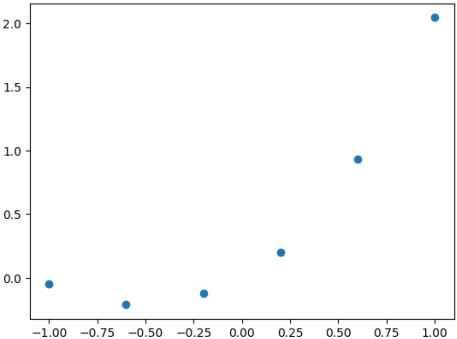
\includegraphics[width=10cm]{problema_interpolazione_esempio.png}
}

Si può risolvere il polinomio di grado $n$ come: 
\[
    p(x) = c_0 + c_1x + c_2x^2 + \dots + c_nx^n    
\]

Per identificare questo polinomio, ordunque, serve \red{calcolare i coefficienti} $c_i, i\in[1,n]$

\subsection{Esistenza dell'unicità}

\teorema{
    $\forall i\in[1,n], \forall (x_i, y_i)$ con $i$ nodi $t_i$, distinti tra loro, esiste un
    unico polinomio di grado minore od uguale a $n$, che indichiamo $P_n(x)$ con e chiamiamo
    polinomio interpolatore dei valori $y_i$ nei nodi $t_i$, tale che
    \[
        p_n(x_i) = y_i,i = 0,\dots, n    
    \]
}

Per la dimostrazione serve prima enunciare un lemma (che non verrà dimostrato)
\lemma{
    Sia $r_n(x)$ un polinomio a coefficienti reali di grado $n$, il numero massimo di zeri distinti è $n$, ovvero:
    \begin{itemize}
        \item Un polinomio di grado $n$ può annullarsi in al massimo $n$ punti distinti.
        \item Se un polinomio di grado $n$ si annulla in più di $n$ punti distinti, allora deve essere il polinomio nullo, cioè identicamente uguale a zero per ogni valore di $x$
        
    \end{itemize}
}

\dimostrazione{
    Assumiamo che esistano due polinomi distinti di grado $n$, ovvero $p_n(x) \text{ e }q_n(x)$ che soddisfino entrambi le relazioni nodali precedenti. La loro differenza $p_n(x) - q_n(x)$ è ovvio verificare che è un polinomio di grado $n$ che si annulla in $n+1$ punti distinti. Per il fatto che il polinomio si annulla in $n+1$ punti e per il lemma enunciato si ha che $p_n(x) - q_n(x) = 0$, quindi $p_n(x) = q_n(x)$. Per assurdo dimostrato

    Q.e.d
}

\subsection{Calcolo del polinomio di interpolazione}

\subsubsection{Metodo classico}
È ovvio verificare che i coefficienti del polinomio di interpolazione di $n+1$ punti $(x_i, y_i)=(x_i, f(x_i))$ si potrebbero calcolare risolvendo il sistema lineare:
\[
    \begin{cases}
        c_0 + c_1x_1 + \dots + c_n x^n_1 = y_1 \\
        c_0 + c_1x_2 + \dots + c_n x^n_2 = y_2 \\
        \cdots \\
        c_0 + c_1x_n + \dots + c_n x^n_n = y_n
    \end{cases}
\]
Tuttavia la matrice dei coefficienti di questo sistema, detta \textbf{matrice di Vandermonde} può essere molto mal condizionata. Inoltre la risoluzione del sistema lineare richiede almeno $O(\frac{n^3}{3})$

\subsubsection{Metodo del polinomio interpolatore di Lagrange}

Introduciamo i polinomi base di lagrange
\definizione{
    Si chiamano \textbf{polinomi base di Lagrange} di grado $n$ particolari funzioni tali che:
    \[
        \phi_k(x_j) = \delta_{k,j}
    \]
    dove $k = j \implies \delta_{k,j}=1$ e $k \neq j \implies \delta_{k,j}=0$
}

La funzione $\phi_k(x)$ può essere scritta come:
\[
    \phi_k(x) = \prod_{j=0, j\neq k} ^ n \frac{x - x_j}{x_k - x_j}
\]
Si può notare, infatti, che include tutti i punti $x_j$ tranne $x_k$, quindi l'indice $j$ percorre tutti gli indici da $0$ a $n$ e nel caso in cui la $x$ in input sia diversa da $x_k$ vi sarà un $x_j$ tale che $x_j = x$, in quel caso il numeratore farà $0$ e renderà nulla la productoria. Nel caso, invece, la $x$ in input sia uguale a $x_k$ avremo $\frac{x_k - x_j}{x_k - x_j} \forall j$ rendendo la productoria uguale ad $1$.

Definito il polinomio posso scrivere il polinomio di interpolazione di Lagrange:
\definizione{
    Si chiama \textbf{polinomio interpolatore di Lagrange} tale funzione:
    \[
        p_n(x) = y_0\phi_0(x) + y_1\phi_1(x) + \dots + y_n\phi_n(x) = \sum_{k=0}^n y_k\phi_k(x)
    \]
}

Infatti soddisfa le condizioni di interpolazione
\[
    p_n(x_i)= \sum_{k=0}^n y_k\phi_k(x_i) = \sum_{k=0}^n y_k\delta_{i,k} = y_i
\]
\subsection{Errore di un polinomio interpolatore di una funzione}

Iniziamo con la definizione di un polinomio interpolatore di una funzione

\definizione{
    Sia $f[0,n] \to \mathbb{R}$ una funzione continua nel suo dominio e sia $y_i = f(x_i), \forall i \in [0,n]$. Sia anche $p_n(x)$ il polinomio interpolatore nei punti $(x_0, y_0), (x_1,y_1), \dots, (x_n, y_n)$

    Allora $p_n(x)$ è detto \textbf{polinomio interpolatore di $f$} e si denota:
    \[
        p_n(f)
    \]

}

Attraverso il polinomio di Lagrange è possibile quantificare l'errore che si commette sostituendo ad una funzione $f$ il suo polinomio interpolante attraverso il seguente teorema

\teorema{
    Sia $I$ un intervallo limitato, e si considerino $n + 1$ nodi di interpolazione distinti $x_i , i = 0, \dots , n$ in $I$. Sia $f$ derivabile con continuità fino all’ordine $n + 1$ in $I$. Allora
    \[
        \forall x \in I. \exists \eta  \in I: E(x) = f(x)- p_n(x) = \frac{f^{n+1(\eta)}}{(n+1)!} \prod_{i=0}^n (x - x_i)
    \] 

    E dove ovviamente $E(x_i) = 0$ dove $i=0,\dots n$
}

l'obbiettivo di questo teorema, quindi, è fornire una formula da cui ricavare un \textbf{errore di interpolazione} $E(x)$, che è la differenza tra la funzione originale $f(x)$ e il polinomio interpolante $p_n(x)$ nei punti in cui non conosciamo il valore esatto di $f(x)$ (ovvero tutti i punti diversi dai nodi)

Da questo \red{teorema non riusciamo a dedurre che}, qualsiasi sia la distribuzione dei
nodi, $max_{x\in I}|E(X)|\to 0$ per $n\to\infty$ ovvero (\red{che il massimo valore dell'errore} $E(x)=f(x)-p_n(x)$ su un intervallo $I$ \red{tende a zero al crescere di  $n$}). Esistono, infatti, alcune funzioni, come la funzione di
Runge, in cui per determinate scelte dei nodi, per esempio equidistanti dove  $max_{x\in I}|E(X)|\to \infty$ per $n\to\infty$. Alla luce di questa considerazione si ha che ad un aumento del grado $n$ del polinomio interpolatore non corrisponde necessariamente un miglioramento nella ricostruzione di una funzione $f$.

\begin{figure}[h!]
    \centering
    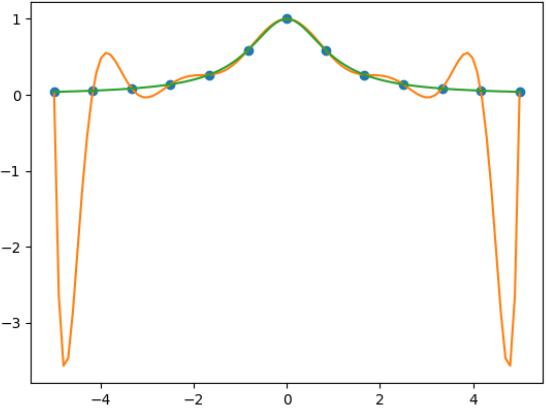
\includegraphics[width=8cm]{runge_interpolato_male.png}
    \caption{In questa immagine troviamo la funzione di Runge (in arancione) e il suo polinomio interpolante (in verde), dove la scelta dei nodi ha causato un errore di interpolazione elevato.}
    \label{fig:runge_interpolazione}
\end{figure}

Il fenomeno di Runge può essere evitato utilizzando opportune distribuzioni di nodi. In
particolare, su un arbitrario intervallo $[a, b]$ consideriamo i cosiddetti \textbf{nodi di Chebyshev-
Gauss-Lobatto}:
\[
    x_i = \frac{a+b}{2} - \frac{b-a}{2} \cos{(\frac{i\pi}{n})} \quad \text{con }i= 0 ,\dots, n   
\]

Notiamo che $x_i = \cos{(\frac{i\pi}{n})}$ se $[a,b] = [-1,1]$. Si può dimostrare che se $f$ è una funzione continua e derivabile con continuità in $[a,b]$ il polinomio interpolante $p_n(x)$ converge a $f(x)$ per $n\to\infty$

\begin{figure}[h!]
    \centering
    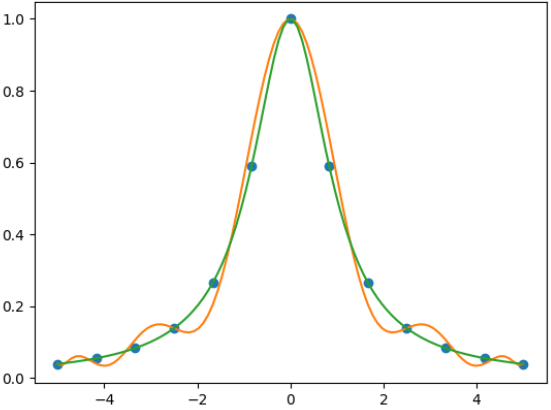
\includegraphics[width=8cm]{runge_interpolato_bene.png}
    \caption{in questa immagina la scelta dei nodi ha causato un errore di interpolazione relativamente basso}
    \label{fig:runge_interpolazione_bella}
\end{figure}

\subsection{Condizionamento dell’interpolazione polinomiale}

Alle volte non si dispone della funzione $f(x_i)$ relativi ai nodi $x_i$, con $i=0,\dots, n$ in un intervallo $I$ ma solo della sua approssimazione, denotata $\tilde{f}(x_i)$. La  perturbazione $f(x_i) - \tilde{f}(x_i)$ potrebbe essere dovuta ad esempio all'effetto degli errori di arrotondamento o ad errori di misura. Se chiamiamo $\tilde{p}_n{x}$ il polinomio interpolatore dei nodi $(x_i, \tilde{f}(x_i))$, si ha:
\[
    \max_{x\in I} |p_n(x) - \tilde{p}_n(x)| = \max_{x\in I}(\sum^n_{i=0}(f(x_i)-\tilde{f}(x_i)\phi_i(x))) =  \Lambda_n (x) \max |f(x_i) - \tilde{f}(x_i)|
\]

Dove $\Lambda_n (x)$ è il numero di condizione che in questo caso è:
\[
    \Lambda_n (x) = \max_{x\in I} |\sum_{i=0}^{n}\phi_i(x)|
\]
Che viene detta \textbf{costante i Lebesgue} che nel caso dell’interpolazione polinomiale su nodi equispaziati la costante di Lebesgue assume il valore:
\[
    \Lambda_n(x) \simeq \frac{2^{n+1}}{n(\log(n) + \gamma) e}    
\]
Dove $\gamma \simeq 5.47721$ è la \textbf{costante di Eulero}. Ciò comporta che per $n$ grande \red{questo tipo di interpolazione potrebbe essere instabile}
\chapter{Problemi inversi}

\section{Problemi diretti}
Nel mondo reale i vari fenomeni sono descritti dalla fisica attraverso un problema diretto come 
\[
    \text{causa} \to \text{modello} \to \text{effetto}     
\]
Per esempio, se voglio calcolare l'accelerazione di un'auto, ne individuo i vari passaggi
\begin{itemize}
    \item La causa: ovvero la forza generata dal motore
    \item Modello: la leggi di newton che forniscono le formule e le leggi apposite (supponendo un sistema inerziale)
    \item Effetto: calcolo dell'accelerazione
\end{itemize}

Quindi acquisisco in input l'origine dell'effetto (ovvero la forza) attraverso un modello (leggi di newton) elaboro questo dato ed infine ne calcolo l'effetto finale (l'accelerazione). In si può scrivere "matematichese": $x \to A \to y$, che traslato in algebra lineare si ha così:
\[
    Ax \to y    
\]
Si giunge così alla definizione di \textbf{problema diretto}
\dfn{}{
Si definisce \textbf{problema diretto} il processo mediante il quale si determina l'effetto dato un sistema e le cause iniziali
}
In altre parole: input -> output

\section{Problemi inversi}

D'altra parte esistono dei casi in cui si riesce solo ad osservare l'effetto di un fenomeno ed occorre, partendo da questo, risalire alla causa, da questo concetto abbiamo la definizione di \textbf{problema inverso}

\dfn{}{
    Un \textbf{problema inverso} è un tipo di problema matematico3 in cui, dato l'effetto o l'output osservato, si cerca di determinare le cause o i parametri del sistema che lo hanno generato
}

Che in termini matematici significa determinare una $x$ conoscendo $A$ e $y$, ovvero output -> input.

Tuttavia \red{nel mondo reale i dati $y$ sono sempre affetti da errore (detto anche \textbf{rumore})} rappresentato dal vettore $\delta$ che non sono solo errori di rappresentazione ma anche legati a problemi di tipo fisico, forti di questa consapevolezza il problema diventa quindi:

\[
    Ax = y+\delta = y^\delta    
\]

\subsection{Problemi inversi lineari con matrici mal condizionate}

Vi sono delle classi di problemi la cui matrice $A$ relativa al modello matematico del problema è mal condizionata, tali problemi si dicono \textbf{mal posti}. In questo caso il problema viene risolto come un problema di minimi quadrati (che permette di avere anche una matrice rettangolare):
\[
    min_x\|Ax - y^\delta\|_2^2
\]

la cui soluzione è
\[
    x^*=\sum_{i=1}^{n} \frac{u^T_iy^\delta}{\sigma_i}v_i    
\]

\subsection{Perturbazione dell'errore}

A causa di un mal condizionamento di $A$ si ha che, in presenza di un errore  $\delta$, si ha che questo errore venga eccessivamente amplificato nella soluzione dei minimi quadrati
\esempio{
    Si consideri una soluzione "vera" (ground truth) denotata con $x_{GT}$ a cui si applica una matrice $A$ che rappresenta il sistema di acquisizione dati per ottenere il vettore $y:Ax = y$ 

    Al vettore $y$ si aggiunge un vettore $\delta$ che rappresenta il rumore e che e’ preso come vettore random da una distribuzione normale con media nulla: $y^\delta = y + \delta$

    Ecco il grafico di questo scempio:
    \begin{center}
        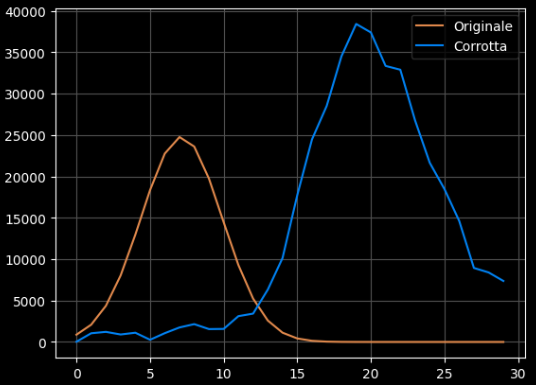
\includegraphics[width=10cm]{img/errore_amplificato.png}    
    \end{center}
    
}

Questo accade perché quando una matrice $A$ è mal condizionata \red{i suoi valori singolari $\sigma_i$ sono molto piccoli, pertanto il numeratore della sommatoria è molto grande}, per capire meglio si osservino i calcoli:
\[
    \min_x\|Ax - y^\delta\|_2^2 = min_x\|Ax - (y+\delta)\|_2^2     
\]
La cui soluzione è:
\[
    x^*=\sum_{i=1}^{n} \frac{u^T_iy^\delta}{\sigma_i}v_i = \sum_{i=1}^{n} \frac{u^T_i(y+\delta)}{\sigma_i}v_i = \sum_{i=1}^{n} \frac{u^T_iy}{\sigma_i}v_i + \sum_{i=1}^{n} \frac{u^T_i\delta}{\sigma_i}v_i
\]

È proprio la seconda sommatoria il problema! È facile verificare che più i $\sigma_i$ sono piccoli più $u^T_i\delta$ è matematicamente "amplificato"
\subsubsection{Condizioni di Picard}
La \textbf{condizione discreta di Picard} è un criterio utilizzato per diagnosticare la "malcondizionatura" nei problemi inversi lineari e per capire la stabilità della soluzione. La condizione discreta di Picard si basa sull'analisi dei \red{valori singolari $\sigma_i$ e i cosidetti coefficienti di Fourier $u_i^Ty^\delta$} 

\dfn{}{
    La \textbf{condizione discreta di Picard} afferma che che, affinché il problema sia ben posto, i coefficienti di Fourier  $u_i^Ty^\delta$devono decrescere almeno altrettanto velocemente dei valori singolari $\sigma_i$
}

\esempio{
    Si consideri questo esempio:
    
    \begin{center}
        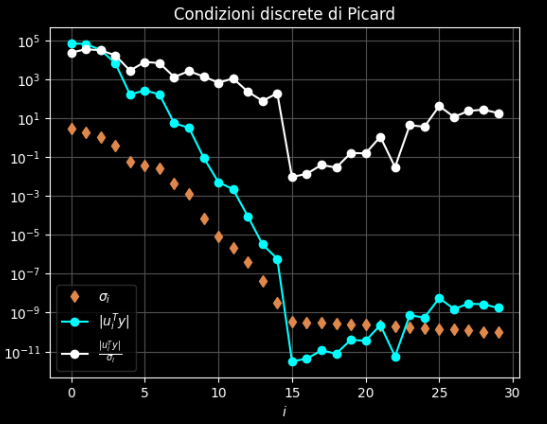
\includegraphics[width=10cm]{img/picard.png}
    \end{center}

    In questo caso la condizione di Picard è rispettata fino all’ indice $i=15$

    Si consideri quest'altro esempio:
    \begin{center}
        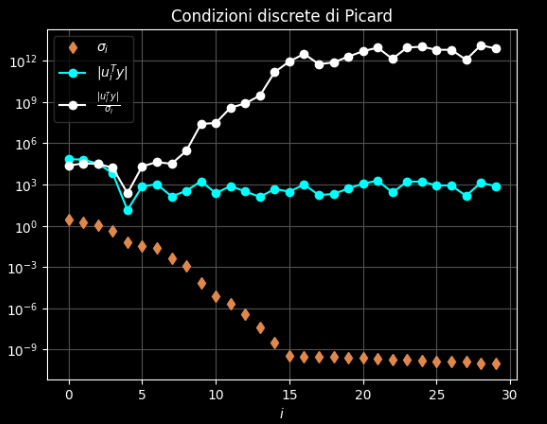
\includegraphics[width=10cm]{img/picard_2.png}
    \end{center} 
    In questo caso la condizione di Picard è rispettata fino all’ indice $i=5$
  
}

\subsection{Metodi di regolarizzazione}
Per affrontare la malcondizionatura e ottenere una soluzione più stabile e accettabile, è \red{necessario modificare il problema attraverso tecniche dette metodi di regolarizzazione}. Esistono diverse tecniche di regolarizzazione, verrano riportate qui sotto

\subsubsection{Decomposizione in Valori Singolari Troncata}

Nel metodo di regolarizazione denominato TSVD (Truncated Singular Value Decomnposition) la soluzione del problema di minimi quadrati: 
\[
    min_x \|Ax - y^\sigma\|_2^2    
\]
viene calcolata come:
\[
    x_{TSVD} = \sum_{i=1}^{K} \frac{u_i^T y^\delta}{\sigma_i} v_i  
\]
Con $K < n$.
Posso anche scrivere la soluzione come:
\[
    x_{TSVD} = \sum_{i=1}^{n} f_i\frac{u_i^T y^\delta}{\sigma_i} v_i  
\]
dove i coefficienti $f_i$ sono detti \textbf{fattori di filtro}, dove in questo caso sono dati da:
\[
    f_i = \begin{cases}
        1 & i\leq K\\
        0 &  i>K
    \end{cases}    
\]

E dove un buon valore $K$ è quello dopo il quale non sono più soddisfatte le condizioni di Picard 

\subsubsection{Regolarizazione di Tikhanov}
La \textbf{regolarizzazione di Tikhonov}, invece, utilizza fattori di filtro che siano numeri in
$[0, 1]$ e che quindi “pesino” le componenti della somma in modo piu’ graduale. In
particolare,\red{ devono essere pesate di più le componenti di indice piccolo, associate ai
valori singolari più grandi, e meno quelle di indice grande, associate ai valori singolari
piu’ piccoli}

Il problema diventa quindi:
\[
    x_{tikh} =  min_x \|Ax - y^\sigma\|_2^2   + \lambda\|Lx\|_2^2
\]
Dove:
\begin{itemize}
    \item $\lambda>0$ è il parametro di regolarizzazione che pesa la parte di congruenza con i dati e la parte di regolarità della soluzione
    \item $L$ è la matrice Identità
\end{itemize}

Si può anche scrivere in questo modo:
\[
    x_{tikh} =  min_x \|Mx - Y\|_2^2 
\]
Dove:\begin{itemize}
    \item $M$ è la matrice di dimensione $2m \times n$ che ha come blocchi in colonna rispettivamente la matrice $A$ e la matrice $\lambda I$
    \item $Y$ è il vettore di dimensione $2m$ che ha
    come vettori colonna rispettivamente $y^\delta$ e il vettore nullo
\end{itemize}

Si può inoltre dimostrare che  la soluzione di Tikhonov posso anche scriverla tramite i fattori di filtro come:
\[
    x_{tikh} = \sum_{i=1}^{n}     f_i \frac{u^T_i y^\delta}{\sigma_i}v_i
\]
dove:
\[
    f_i = \frac{
        \sigma^2_i
    }{
        \sigma^2_i + \lambda  
    }
\]
\subsubsection{Principio di maassima discrepanza}

Si giunge, tuttavia, ad un problema: la scelta del parametro di regolarizzazione nel metodo di Tikhonov. Infatti questa scelta è sicuramente la parte piu’ delicata della
regolarizzazione, un parametro troppo piccolo non
toglie il rumore dalla soluzione, mentre un parametro troppo grande produce una
soluzione troppo regolare, in cui non e’ piu’ presente il rumore ma per esempio le
oscillazioni o i picchi che ci sono nella soluzione esatta vengono troppo ridotti.

\red{Teoricamente il valore ottimale del parametro $\lambda_{opt}$ è quello che minimizza:}
\[
    \lambda_{opt} = \min_\lambda\|x_\lambda - x_{GT}\|_2^2
\]
dove $x_\lambda$ è la soluzione calcolata in corrispondenza di un certo $\lambda$.

Non esiste un metodo sempre efficiente per scegliere il parametro di regolarizzazione.
Sicuramente in pratica spesso si usa una tecnica euristica che consiste nel provare
alcuni parametri e scegliere quello che produce la soluzione che ci sembra migliore (trial and test). La tecnica sicuramente più utilizzata in pratica è il principio di massima discrepanza.

\dfn{}{
    Il \textbf{Principio di Massima Discrepanza} afferma che il parametro di regolarizzazione $\lambda$ dovrebbe essere scelto in modo tale che la norma del residuo (cioè la differenza tra i dati osservati e quelli ricostruiti) sia proporzionale alla stima della norma del rumore nei dati

    Formalmente:
    \[
        \|Ax_\lambda - y^\delta \| = v_{DP} |\delta|_2^2
    \]
    Dove: 
    \begin{itemize}
        \item $x_\lambda$ è la soluzione regolarizzata con parametro $\lambda$
        \item $v$ è un fattore di proporzionalità (spesso scelto vicino a 1)
        \item $\|\delta\|$ è la norma dell'errore (spesso è impossibile conoscerla ma si può fare una stima)
    \end{itemize}
}

Quindi \red{il residuo deve essere uguale alla norma del rumore, quindi provo tanti $\lambda$, quello più vicino a questa soluzione è quello migliore}


\chapter{immagini}
Un problema piuttosto complesso è la conversione di una immagine da analogica a digitale che, ovviamente, deve essere gestita tramite i pixel. Astraendo matematicamente un'immagine, infatti, è possibile trarre una matrice $M\times N$ che rappresenta i vari pixel ed i suoi coefficienti, ai fatti, rappresentano quali sfumature di colore verranno mostrate ed in quale posizione. Tuttavia se un'immagine di grigi è rappresentabile da un'unica matrice che avrà come coefficienti soltanto valori interi da un minimo di 0 ad un massimo di
255 ( 0 rappresenta il colore nero e 255 rappresenta il colore bianco), un'immagine a colore è ottenuta tramite la sovrapposizione di tre rappresentazioni della stessa immagine: una in scala di rossi, una in scala di verdi ed una in scala di blu; sarà quindi richiesto che il colore di ogni pixel di questa immagine sia rappresentato da vettore di tre valori, ciascuno per ogni intensità del colore rosso, verde e blu

\definizione{
    Sia $A\in \mathbb{R}^{M\times N}$ e sia $k\in \mathbb{N}$, diremo che: una matrice $B$ di dimensioni $(M+2k)\times (N+2k)$ \textbf{estende} la matrice $A$ se e solo se vale:
    \[
        \forall (i,j)\in \{\,\dots,M\}\times \{1,\dots, N\}. A_{(i,j)} = B_{(i+k, j+k)}
    \] 
}

Esempietto:
\esempio{
    
    \[A=  
        \begin{pmatrix}
            7&8&9\\
            12&13&14\\
            17&18&19
        \end{pmatrix}    
    \]
    Si può affermare che che la seguente matrice
    \[A=  
        \begin{pmatrix}
            1&2&3&4&5\\
            6&7&8&9&10\\
            11&12&13&14&15\\
            16&17&18&19&20\\
            21&22&23&24&25
        \end{pmatrix}    
    \]
    estende $A$, dove si ha $k=1$
}
Chiaramente, per ogni matrice ne esistono infinite che la estendono
\definizione{
    Sia $K\in\mathbb{R}^{D\times D}$ con $D$ dispari. Si definisce il \textbf{centro di matrice} della matrice $K$ come l'elemento di coordinate $(\frac{D+1}{2}, \frac{D+1}{2})$
}
\esempio{
    Sia la matrice di dimensioni $5\times 5$
    \[
       A=\begin{pmatrix}
        1&2&3&4&5\\
        6&7&8&9&10\\
        11&12&13&14&15\\
        16&17&18&19&20\\
        21&22&23&24&25
    \end{pmatrix} 
    \]
    
    Il suo centro di matrice è $(\frac{5+1}{2}, \frac{5+1}{2}): = 13$
}

\definizione{
    Sia $A\in\mathbb{R}^{M\times N}$ e sia $B\in\mathbb{R}^{(M+(D-1))\times (N+(D-1))}$ con $D$ dispari che estenda $A$. $\forall(i,j)\in\{1,\dots, M\}\times\{1,\dots, N\}$ si definisce $W_{(i,j)}\in\mathbb{R}^{D\times D}$ si definiscono \textbf{sotto-matrici} di $B$, il cui centro è $B_{(i + \frac{D-1}{2}, j + \frac{D-1}{2})}$
}
\esempio{
    Sia $A\in\mathbb{R}^{3\times 3}$
    
    \[
        \begin{pmatrix}
            7&8&9\\
            12&13 &14\\
            17&18&19
        \end{pmatrix}
    \]

    Occorre trovare una matrice $(3 + (D - 1)) \times (3 + (D - 1)) = (3 + 2) \times (3 + 2)$ che estenda $A$, ad esempio:
    \[
        \begin{pmatrix}
            1&2&3&4&5\\
            6&7&8&9&10\\
            11&12&13&14&15\\
            16&17&18&19&20\\
            21&22&23&24&25
        \end{pmatrix}
    \]

    ne segue che, per esempio, la matrice $W_{(1,3)}$ è la sotto-matrice di $B$, di dimensioni $3 \times 3$, il cui centro sia $B_{(2,4)}$. Di seguito:

    \[
        W_{(1,3)}  = \begin{pmatrix}
            3&4&5\\
            8&9&10\\
            13&14&15
        \end{pmatrix}    
    \]
}

\definizione{
    Sia $A\in \real^{M \times N}$ e $K\in\real^{D \times D}$, con $D$ un numero naturale dispari. Sia $B$ una matrice di dimensioni $(M + (D - 1)) \times (N + (D - 1))$ che estenda $A$. $\forall (i,j)\in \{1, … , M\} \times \{1, … , N\}$, siano $W_{(i,j)}$ le sotto-matrici di dimensione $D\times D$ definite precedentemente.

    Definiamo la matrice $C\in\real^{M\times N}$, come segue:
    \[
        \forall(i,j) \in    \{1, … , M\} \times \{1, … , N\}: C_{i,j} = \sum_{m=1}^{\frac{D-1}{2}}\sum_{n=1}^{\frac{D-1}{2}} K(m,n) W_{(i,j)}(m,n)
    \]
    Tale matrice $C$, che verrà anche denotata con $C = [K * A | B]$, è chiamata \textbf{convoluzione} di $K$ e $A$ rispetto all’estensione $B$

    All’interno del contesto di questa definizione, la matrice $K$ prenderà il nome di \textbf{nucleo} di convoluzione o kernel di convoluzione
}

\section{Estensione di una matrice}

\definizione{
    Sia $k$ un numero naturlae e $B$ una matrice di dimensioni $(M + 2k) \times (N + 2k)$. Definiamo la funzione:
    \[
        \mathcal{P}:\real^{M\times N}\to \real^{(M+2k)\times (N+2k)}\quad X\to \mathcal{P}(X)
    \]
    Tale che:
    \[
        \forall(i,j) \in    \{1, … , M\} \times \{1, … , N\}: X_{(i,j)} = \mathcal{P}(X)_{(i+k, j+k)}
    \]
    e:
    \begin{itemize}
        \item le prime $k$ colonne di $\mathcal{P}(X)$ siano uguali alle prime $k$ colonne di $B$
        \item le ultime $k$ colonne di $\mathcal{P}(X)$ siano uguali alle ultime $k$ colonne di $B$
        \item le prime $k$ righe di $\mathcal{P}(X)$ siano uguali alle prime $k$ righe di $B$
        \item le ultime $k$ righe di $\mathcal{P}(X)$ siano uguali alle ultime $k$ righe di $B$
    \end{itemize}
    La funzione $P$ così definita prenderà il nome di \textbf{patter di estensione di ordine $k$ rispetto alla matrice $B$}
}
È chiaro che, per come è definita la funzione $\mathcal{P}(X)$, questa estenderà sempre la matrice $X$

\definizione{
    Definiamo \textbf{funzione di convoluzione} la seguente:
    \[
        [K*(\cdot)|\mathcal{P}]:\real^{M\times N}\to \real^{M\times N} \quad X\to [K*X|\mathcal{P}(X)]   
    \]
    \begin{itemize}
        \item Dove $K$ è un nucleo di convoluzione di dimensioni $D\times D$ fissato
        \item $\mathcal{P}$ è un pattern di estensione di ordine $\frac{D-1}{2}$, rispetto ad una qualche matrice $B\in\real^{(M+(D+1)\times N + (D-1))}$, sempre fissata 
    \end{itemize}
}
\esempio{
    Si prendi come esempio tale immagine
    \begin{center}
        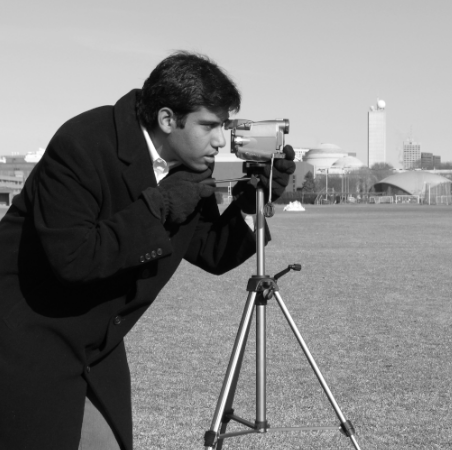
\includegraphics[width=7cm]{bro_foto.png}
    \end{center}
    E si supponi sia una matrice $A$ e si supponga tale matrice abbia, come nucleo di convoluzione $K$, tale matrice:
    \[
        K=\begin{pmatrix}
            0&\frac{1}{4}&0\\
            \frac{1}{4}&0&\frac{1}{4}\\
            0&\frac{1}{4}&0
        \end{pmatrix}    
    \]
    Ora non resta che svolgere la convoluzione in sè. 
    Ecco come:
    \begin{itemize}
        \item consideriamo una sotto-matrice $W$, sempre di dimensioni $D \times D$, della matrice $B$
        \item svolgiamo il prodotto scalare fra: la prima colonna di $W$ e la prima riga di $K$ , la seconda colonna di $W$ e la seconda riga di $K$ , così via fino alla \textit{D}-esima colonna di $W$ e alla \textit{D}-esima riga di $K$
        \item sommiamo tutti i prodotti scalari ottenuti
        \item il valore così determinato, diventerà il valore del pixel al centro della sotto-matrice $W$ considerata
        \item ripetere per tutte le sotto-matrici
        \item rimuovere le condizioni al bordo
    \end{itemize}
    \begin{center}
        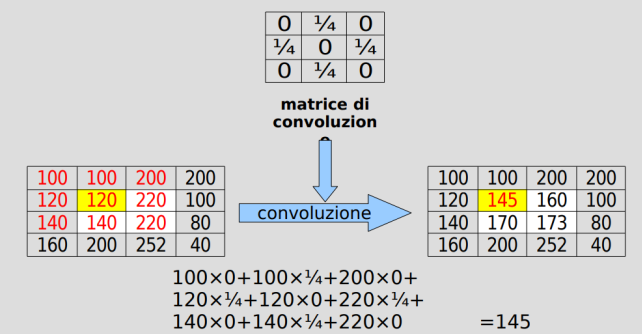
\includegraphics[width=7cm]{convoluzione_zio_pera.png}
    \end{center}
    In questo caso, il kernel utilizzato sostituisce il valore di ogni pixel con la media aritmetica dei valori contenuti nei quattro pixel ad esso adiacenti

    Ottenendo il seguente effetto di sfocatura:
    \begin{center}
        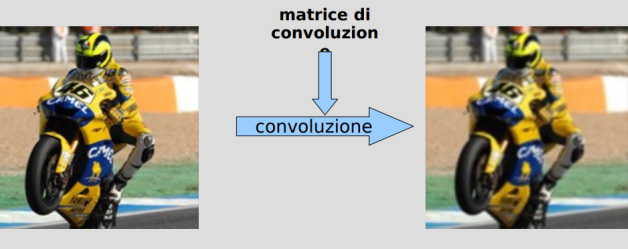
\includegraphics[width=7cm]{sfocatura.png}
    \end{center}

    Se si considera, invece, il seguente kernel:
    \[
        K = \pmatrix{
            0&1&0\\
            1&-4&1 \\
            0&1&0
        }  
    \]
    Osserviamo che, poiché la somma dei coefficienti è 0, sappiamo che se un pixel ha approssimativamente lo stesso colore dei quattro che gli sono adiacenti, allora verrà rimpiazzato da un valore prossimo a zero; in altre parole, il pixel diverrà di colore nero.
    Ne segue che tutti e soli i pixel che avranno un valore non nullo, saranno quelli posizionati in mezzo a due regioni di colori contrastanti. Pertanto, questo è un filtro che evidenzia i bordi dell’immagine
    \begin{center}
        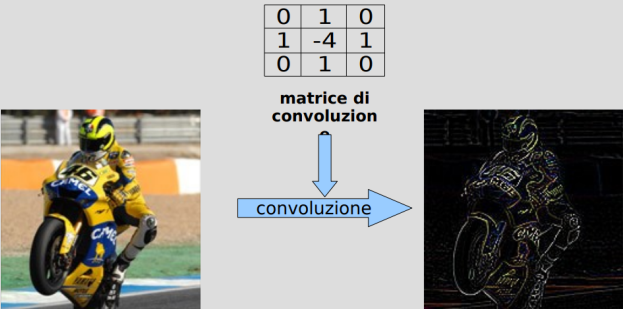
\includegraphics[width=7cm]{bordizzatura.png}
    \end{center}
}

\section{Point Spread Function}
Nel momento in cui un macchinario sensibile alla luce si accinge a fotografare, per esempio, ad una fonte luminosa puntiforme del tipo:
%TODO fai foto catso

Si ha che l'imagine ottenuta sarà:
%TODO fai foto dio pene

L'immagine che si ottiene è, quindi, un allargamento della fonte luminosa centrata nella fonte puntiforme. Questo fenomeno \red{è del tutto deterministico e legato all'apperacchiatura utilizzata per catturare l'immagine}. 

Sia $X$ la prima immagine e $Y$ la seconda, matematicamente si ha che:
\[
    A(X) = Y    
\]
Dove $\mathcal{A}$ è una funzione chiamata \textbf{Point Spread Function}. Ad essere più precisi riporterò qui la definizione di Point Spread Function
\definizione{
    Sia $x$ un immagine che rappresenta perfettamente il nostro
    oggetto originale. È definita $\mathcal{A}$ Point Spread Function, tale funzione:
    \[
        \mathcal{A}(x) = [K * x | \mathcal{P}]    
    \] 
    Dove $K$ è un kernel di convoluzione e $\mathcal{P}$ è un pattern di estensione
}

\subsection{PSF con errori non deterministici}
Tuttavia gli errori non deterministici non sono solo gli unici errori che corrompono le immagini, nel corso dell’acquisizione dell’immagine fenomeni aleatori e sostanzialmente imprevedibili danneggiano ulteriormente la nitidezza dell’immagine ottenuta.

Adesso sia $w$ un immagine i cui valori dei pixel siano stati selezionati aletoriamente secondo la distribuzione del rumore Gaussiano bianco. 

Si ha, quindi, un modello matematico \textbf{discreto} che spieghi come si sia formulata l'immagine $g$ (quella restituita dal nostro sistema di formazione di immagini), a partire da $x$, l'immagine che rappresenta veramente l'oggetto:
\[
    y^\delta = \mathcal{A}(x) + w =  [W*x|\mathcal{P}] + w  
\]
dove: 
\begin{itemize}
    \item $K$ è un qualche kernel di convoluzione
    \item $P$ è un pattern di estensione 
    \item $w$ è il medesimo di cui sopra
    \item $\mathcal{A}$ è la point spread function
\end{itemize}

Alternativamente si piò riscrivere il modello nella seguente forma matriciale:
\[
    y^\delta = Ax + w    
\]
Dove $A\in\real^{M\times N}$ che contiene le informazioni del nucleo
di convoluzione ed è tale che:
\[
    Ax = K * x
\]

Adesso ovviamente si vuole ardentemente sapere l'immagine originale $x$ zio pera
\subsubsection{Soluzione naive}
La soluzione naive è quella ottenuta risolvendo il problema di minimi quadrati:
\[
    min_x \|Ax-y^\delta\|_2^2    
\]
Essendo la matrice A di dimensione non molto piccola, calcolare la soluzione con la SVD è troppo costoso (ricordiamo che la complessità computazionale della fattorizzazione SVD è $O(4/3mn^2 )$ per una matrice di dimensione $m*n$). Quindi si risolvono le equazioni
normali:
\[
    A^TAx=A^Ty^\delta    
\]
Il sistema ha matrice simmetrica e definita positiva (supponiamo A di rango massimo) e per ragioni computazionali è conveniente utilizzare un metodo iterativo. Quindi  si applichiamo il CGLS al sistema delle equazioni normali
\subsection{Metriche di valutazione}
Le \textbf{metriche di valutazione} sono strumenti matematici utilizzati per quantificare la qualità di una ricostruzione, come nel caso della ricostruzione di un'immagine. Servono per confrontare un'immagine ottenuta (ricostruita) con il "ground truth" (l'immagine originale), con l'obiettivo di avere un numero che rappresenti quanto la ricostruzione sia accurata o fedele rispetto all'originale. Ci sono diverse metriche, proprio per avere diversi punti di vista
\subsubsection{errore relativo}
\definizione{
    siano $x_{GT}$ il "ground truth" e $x$ l'immagine ricostruita, viene definito l'errore relativo $ER$ tale valore:
    \[
        ER= \frac{\| x - x_{GT} \|_2^2}{\| x_{GT} \|_2^2}

    \]
}
\subsubsection{Rapporto Segnale-Rumore di Picco}
Prima di definire il Rapporto Segnale-Rumore di Picco occorre prima deifinire \textbf{l'errore quadratico medio} 
\definizione{
    Siano $M$ e $N$ le dimensioni dell'immagine, si definisce \textbf{ l'Errore Quadratico Medio} il seguente valore:
    \[
        MSE = \frac{\|x-x_{GT}\|_2^2}{MN}
    \]
}
Questo valore misura la differenza media al quadrato tra i pixel dell’immagine originale e quelli della ricostruzione. adesso si può introdurre il PSNR

\definizione{
    Sia $\max_{i,j}|x_{i,j}|$ è il valore massimo dell’immagine ricostruita (ad esempio, 255 per immagini in scala di grigi a 8 bit) e $MNE$ l'errore quadratico medio, si definisce \textbf{Rapporto Segnale-Rumore di Picco} tale valore:
    \[
        PSNR = 10 \cdot \log_{10}{(\frac{(\max_{i,j}|x_{i,j}|)^2}{MSE})}    
    \]
}
Un valore di PSNR più alto indica una qualità della ricostruzione migliore, perché significa che la differenza tra l'immagine ricostruita e l'originale è bassa

\subsubsection{Indice di Similarità Strutturale (SSIM)}
Il Structural Similarity Index (SSIM) è una metrica più complessa, progettata per essere più coerente con la percezione visiva umana. Considera non solo le differenze di intensità dei pixel, ma anche la struttura, luminanza e contrasto delle immagini. In altre parole, valuta quanto due immagini sono simili in termini di caratteristiche visive piuttosto che pixel per pixel. Più è vicino a uno, migliore è la qualità dell’immagine

\subsubsection{Roba}
\definizione{
    Sia \( A \) una matrice \( M \times N \), definiamo la funzione \( \mathcal{L} : \mathbb{R}^{M \times N} \rightarrow \mathbb{R}^{N \ast M} \) come segue:

\[
\mathcal{L}(A)
\]
è un vettore di dimensione \( N \ast M \), le cui:
\begin{itemize}
    \item prime \( N \) componenti sono la prima riga di \( A \), letta da sinistra a destra;
    \item seconde \( N \) componenti sono la seconda riga di \( A \), letta da sinistra a destra;
    \item \(\dots\)
    \item \( M \)-esime \( N \) componenti sono la \( M \)-esima riga di \( A \), letta da sinistra a destra.
\end{itemize}

Analogamente si definisce la conversione lessicografica per colonne.

}

\subsection{Regolarizzazione di Tikhonov applicata alle immagini}
Durante la soluzione di Naive si considerava il problema delle immagini come il seguente problema di minimo:
\[
    \min_x \|\|_2^2    
\]

Tuttavia dato che si ha un errore $y^\delta$ è necessario stabilizzare la funzione col metodo di regolarizzazione di Tikhonov:
\[
    \min_x \|Ax-y^\delta\|_2^2 + \lambda\|x^2\|_2^2
\]
Dove $\lambda$ è il parametro di Regolarizzazione. Applicando le condizioni del primo ordine $\nabla (f) = 0$ si ha:
\[
    (A^T A + \lambda I)x = A^T y^\delta    
\]

È possibile quindi risolvere il problema tramite il metodo CGLS
\subsubsection{Regolarizzazione con Variazione totale}
Una funzione di regolarizzazione alternativa a quella di Tikhonov e molto utilizzata nell’imaging è la funzione di Variazione Totale (TV) definita in questo modo:

\[
    TV(x) = \|\nabla (x)\|_1 = \sum_{i=1}^{M}\sum_{j=1}^{n} \sqrt{(x_{i+1,j}- x_{i,j})^2 + (x_{i,j+1 - x_{i,j}})^2}    
\]

La funzione $TV$ non è differenziabile nel punto $(0,0)$. Per ottenre la differenziabilità, si inserice un piccolo parametro $\beta > 0$:
\[
    TV^\beta(x) = \sum_{i=1}^{m}\sum_{j=1}^{n} \sqrt{(x_{i+1,j}- x_{i,j})^2 + (x_{i,j+1} - x_{i,j})^2 + \beta^2}
\]

Dove i valori di solito utilizzati per $\beta$ sono nell'ordine di $10^{-3}$

Il problema di regolarizzazione diventa quindi:
\[
    \min_x \|Ax-y^\delta\|_2^2 + \lambda TV ^ \beta(x)    
\]
Il metodo di regolarizzazione con TV ha il vantaggio di essere particolarmente efficace nell’eliminare il rumore e allo stesso tempo meglio preservare i contorni, anche in caso di basso rapporto segnale/rumore. Il suo uso è motivato dalla sua abilità nel recuperare le discontinuità nell’immagine, inoltre preserva i bordi dell’immagine rimuovendo piccoli dettagli come il rumore.
All’aumentare del parametro di regolarizzazione l’immagine tende a una immagine costante a tratti



\end{document}
